%
% Sample SBC book chapter
%
% This is a public-domain file.
%
% Charset: ISO8859-1 (latin-1) áéíóúç
%
\documentclass[../main.tex]{subfiles}
\graphicspath{{\subfix{../figures/}}}

\begin{document}
\chapter{{Limitations} of composability of cis-regulatory elements in messenger RNA}

\section{Chapter 4 Introduction}

\subsection{Discovering sequence determinants of gene expression}

Since the beginning of molecular biology, biologists struggled to explain the size of the genomes of eukaryotes as it was quickly understood that only a fraction directly encoded protein sequences \parencite{MIRSKY1951, Thomas1971}. 
Around the same time, scientists were discovering that RNA and protein synthesis within cells can be regulated by hormones \parencite{Ui1963}.
In addition, investigations in to the lac operon discovered the promoter as a sequence adjacent to a coding sequence which regulated expression through the initiation of transcription \parencite{JACOB1964}.
All of this work led to the theory that a significant portion of the non-coding genome was dedicated to the regulation of expression. 
The theory included the classification of sequences that either affect the expression of its own gene; for example, promoters, or signal changes in expression of other genes; for example, hormones \parencite{Britten1969}. 

Today, these two types of regulatory sequence are called cis-regulatory elements (CRE) and trans-regulatory elements.
Massively parallel approaches now characterise smaller CREs by exploring a large library of promoter elements with a single terminator \parencite{Sharon2012}, or conversely a library of terminators with a single promoter \parencite{Shalem2015}.
Cis-regulatory element include: sequences imbuing mRNA secondary structures, RNA binding protein motifs, and enhancer regions \parencite{Li2015}. 
The possible effects of regulatory elements has also been expanded to include contributions to localisation, degradation, and translation.
Meanwhile, trans-regulatory elements include: transcription factors \parencite{Spitz2012}, the sliceosome \parencite{Will2011}, and ribonucleoproteins \parencite{Bleichert2010}.
However, the line between trans- and cis- regulatory elements is becoming increasing blurred \parencite{Savarese2006}.

%\subsubsection{finding motifs}
%Bioinformatics Approaches to Gain Insights into cis-Regulatory Motifs Involved in mRNA Localization %https://link.springer.com/chapter/10.1007/978-3-030-31434-7_7

%Localization elements and zip codes in the intracellular transport and localization of messenger RNAs in Saccharomyces cerevisiae
%https://wires.onlinelibrary.wiley.com/doi/10.1002/wrna.1591

Computational methods continued to be developed for the discovery and quantification of cis-regulatory elements, such as sequence motifs recognised by regulatory proteins.
Prominent methods for mapping CRE sequence-function relationships include predicting functional data with short sequence features, often using linear models \parencite{Shalgi2005,Cheng2017,Vijayabaskar2019} or, directly comparing the sequences of genes with similar characteristics to determine the presence of short
consensus sequence motifs \parencite{Hogan2008,Kretz2013} using motif discovery software \parencite{Elemento2007,Bailey2015}.
Both of these approaches make the implicit approximation that the contribution of a short CRE is independent of context, so that the effect of combining motifs is composed of a linear sum (on the appropriate scale) of the individual CRE contributions.
The approximation that short CREs act independently helps to find elements that have clear contributions, and to simplify a vast search space that would be made exponentially larger by accounting for CRE interactions. 
However, framing the search for CREs around independent contributions from short motifs overlooks multi-part motifs, interactions between motifs, and that motifs may be active only in specific contexts.

\subsection{From regulatory elements to modular cloning.}

The discovery of regulatory elements with predictable contributions to gene expression opened the door to the idea of creating synthetic genes.
Technology developed over the later half of the 20th century has turned the creation of synthetic genes into an industry.
First, the discovery of restriction enzymes allowed the precise cutting of DNA using designed recognition sites. 
The original type I restriction enzyme, which cut within the recognition site, \parencite{Arber2003,Meselson1968} was followed by the more useful type II restriction enzyme, which cut a few base pairs upstream of the recognition site \parencite{Smith1970,Kelly1970}. 
Next, the understanding of the recombination mechanisms enabled the pasting of multiple different segments of DNA together \parencite{Jackson1972,Cohen1973}. 
Then, ten years after the discovery of promoters scientists transformed E.coli cells with a synthetic, replicating plasmid which expressed resistance to the antibiotic tetracycline \parencite{Cohen1973}. 
The tools for separating and combining segments of DNA into replicating plasmids laid the ground work for integrate-able cassettes of interchangeable genetic parts and the origins of modular cloning.
Up to then work was mostly completed in prokaryotes, but work to efficiently transform yeast \parencite{Beggs1978} and later mammalian cells \parencite{Capecchi1989} enabled access to more complex synthesis machinery and to more complex proteins. 
The creation of polymerase chain reaction dramatically increased the efficiency of transforming organisms and accessing new genes as regions of genomes could be selected and amplified by designing primers \parencite{Saiki1988}. 
The invention and improvement of these tools culminated in the creation of synthetic circuits and regulatory elements at the turn of century \parencite{Elowitz2000,Gardner2000}.

The last 20 years of pioneering synthetic biology research as been defined by the standardisation of libraries of regulatory parts. 
BioBricks is the de facto library of choice that pioneers the "pick and mix" paradigm \parencite{Knight2003}.
Shifting the focus from fundamental cell biology to metabolic engineering, users no longer needed to understand the specifics genomes to find suitable regulatory parts, but instead focus on the end product. 
Bioengineering is quickly becoming a staple of industry with production of high value compounds with high yields reduced waste \parencite{Krivoruchko2015}.
Genetically modified organisms have now been created to detect oil spills, arsenic in water and even the presence of specific viruses \parencite{Wan2019,Willardson1998,Tancharoen2019}.

Intrinsic to the success of synthetic biology is the development of modular processes to assemble genetic parts \parencite{Curran2013,Lee2015,Garcia2018,Andreou2018}.
Several groups have constructed standardised libraries comprising promoter (including 5’UTR) and terminator (including 3’UTR) parts, which can be combined to achieve desired expression of synthesized proteins.
The characterisation of all possible promoter-terminator pairings is impractical, so standardised libraries generally characterise parts independently, for example testing many promoters with the same coding sequence and terminator \parencite{Lee2015}.
Because these experiments do not measure interactions between different parts, they rely on the untested assumption that those parts have more or less identical effects across different contexts.
The majority of interactions between parts are negligible, but unpredictable behaviour at crucial stages of genetic pathways continue to hamper synthetic biology projects \parencite{Kittleson2012}.

\subsection{Current limitations in predicting gene expression}

The unpredictability of expression in the expression of synthetic constructs highlights the current limitations in our understanding of gene expression.
Currently, the most common solution to this problem is to take advantage of the scale of high throughput assays now available. 
Automation of construct transformation, growth and characterisation is enabling tonnes of variants to be compared at the same time point. 
Together with high throughput RNA-Seq and flow cytometry thousands of constructs can be tested and those that behave as expected can be picked \parencite{Kosuri2013}. 
However, this remains a costly and high expertise endeavour that highlights how much there remains to be understood about gene regulation. 

Meanwhile, the continued development of statistical models to accurately predict gene expression from DNA sequences offers another route to better predict behaviour without needing to conduct additional experiments \parencite{Li2015}. 
However, many CRE finding algorithms tend to rely on models of independent effects, that is, composability.
Meanwhile, more complex models that can account for non-linear interactions typically hide their decision making. 
Interpreting the decisions made from "black box" machine learning algorithms \parencite{Guidotti2018} could be significant in understanding the biological mechanisms through which gene expression is regulated. 
Understanding gene regulation pathways requires more balanced approach that enables interactions but in an interpretable way. 

Here, we explore the limitations of composability beyond regulatory regions with a focus on interactions between regulatory sequence motifs.
We first show the changing regulatory behaviour of terminator sequences paired with different promoters and coding sequences.
We measure the fluorescence of 120 chimera constructs and highlight the irregular but significant changes in gene expression between contexts. 
Then, we investigate whether the changes in regulatory behaviour are reflected in the cis-regulatory elements within these regions. 
We conduct an analysis of contributions to half life from suspected cis-regulatory elements using published data sets and create a shortlist of motifs of interest.
Then, we show that these motifs on their own have different contributions to gene expression depending on context. 
Finally, we confirm motifs contributions to gene expression using RNA-Seq experiments and explore possible positional effects on motif behaviour. 
 
\section{Chapter 4 Results}

\subsection{Terminator effects on gene expression depend on cis-regulatory context}

To investigate the context dependence of terminator regions, we created a library of 120 constructs (Figure \ref{fig:pro-ter-platereader-mCherry-mTurq-norm}A), containing all combinations of 6 promoters (including 5'UTR), 2 coding sequences, and 10 terminators (including 3'UTR).
We selected promoters and terminators from native yeast genes spanning a variety of different expression patterns and functions (Table \ref{tab:terminator-summary-table}).
To choose specific sequence lengths for the terminators of our constructs, we referred to published measurements of median 3'UTR length \parencite{Pelechano2013} because sequences that are necessary and sufficient for efficient transcriptional termination are found upstream of the termination site \parencite{Guo1996}.
For terminators with measured length under 200nt, we used the standardised parts length of 200nt from the YeastFab library.
The 2 coding sequences (CDS) expressed mCherry or mTurquoise2 fluorescent proteins, which are bright fluorophores with only 30\% amino acid identity \parencite{Shaner2004, Goedhart2012}.



\begin{figure}[p]

{\centering 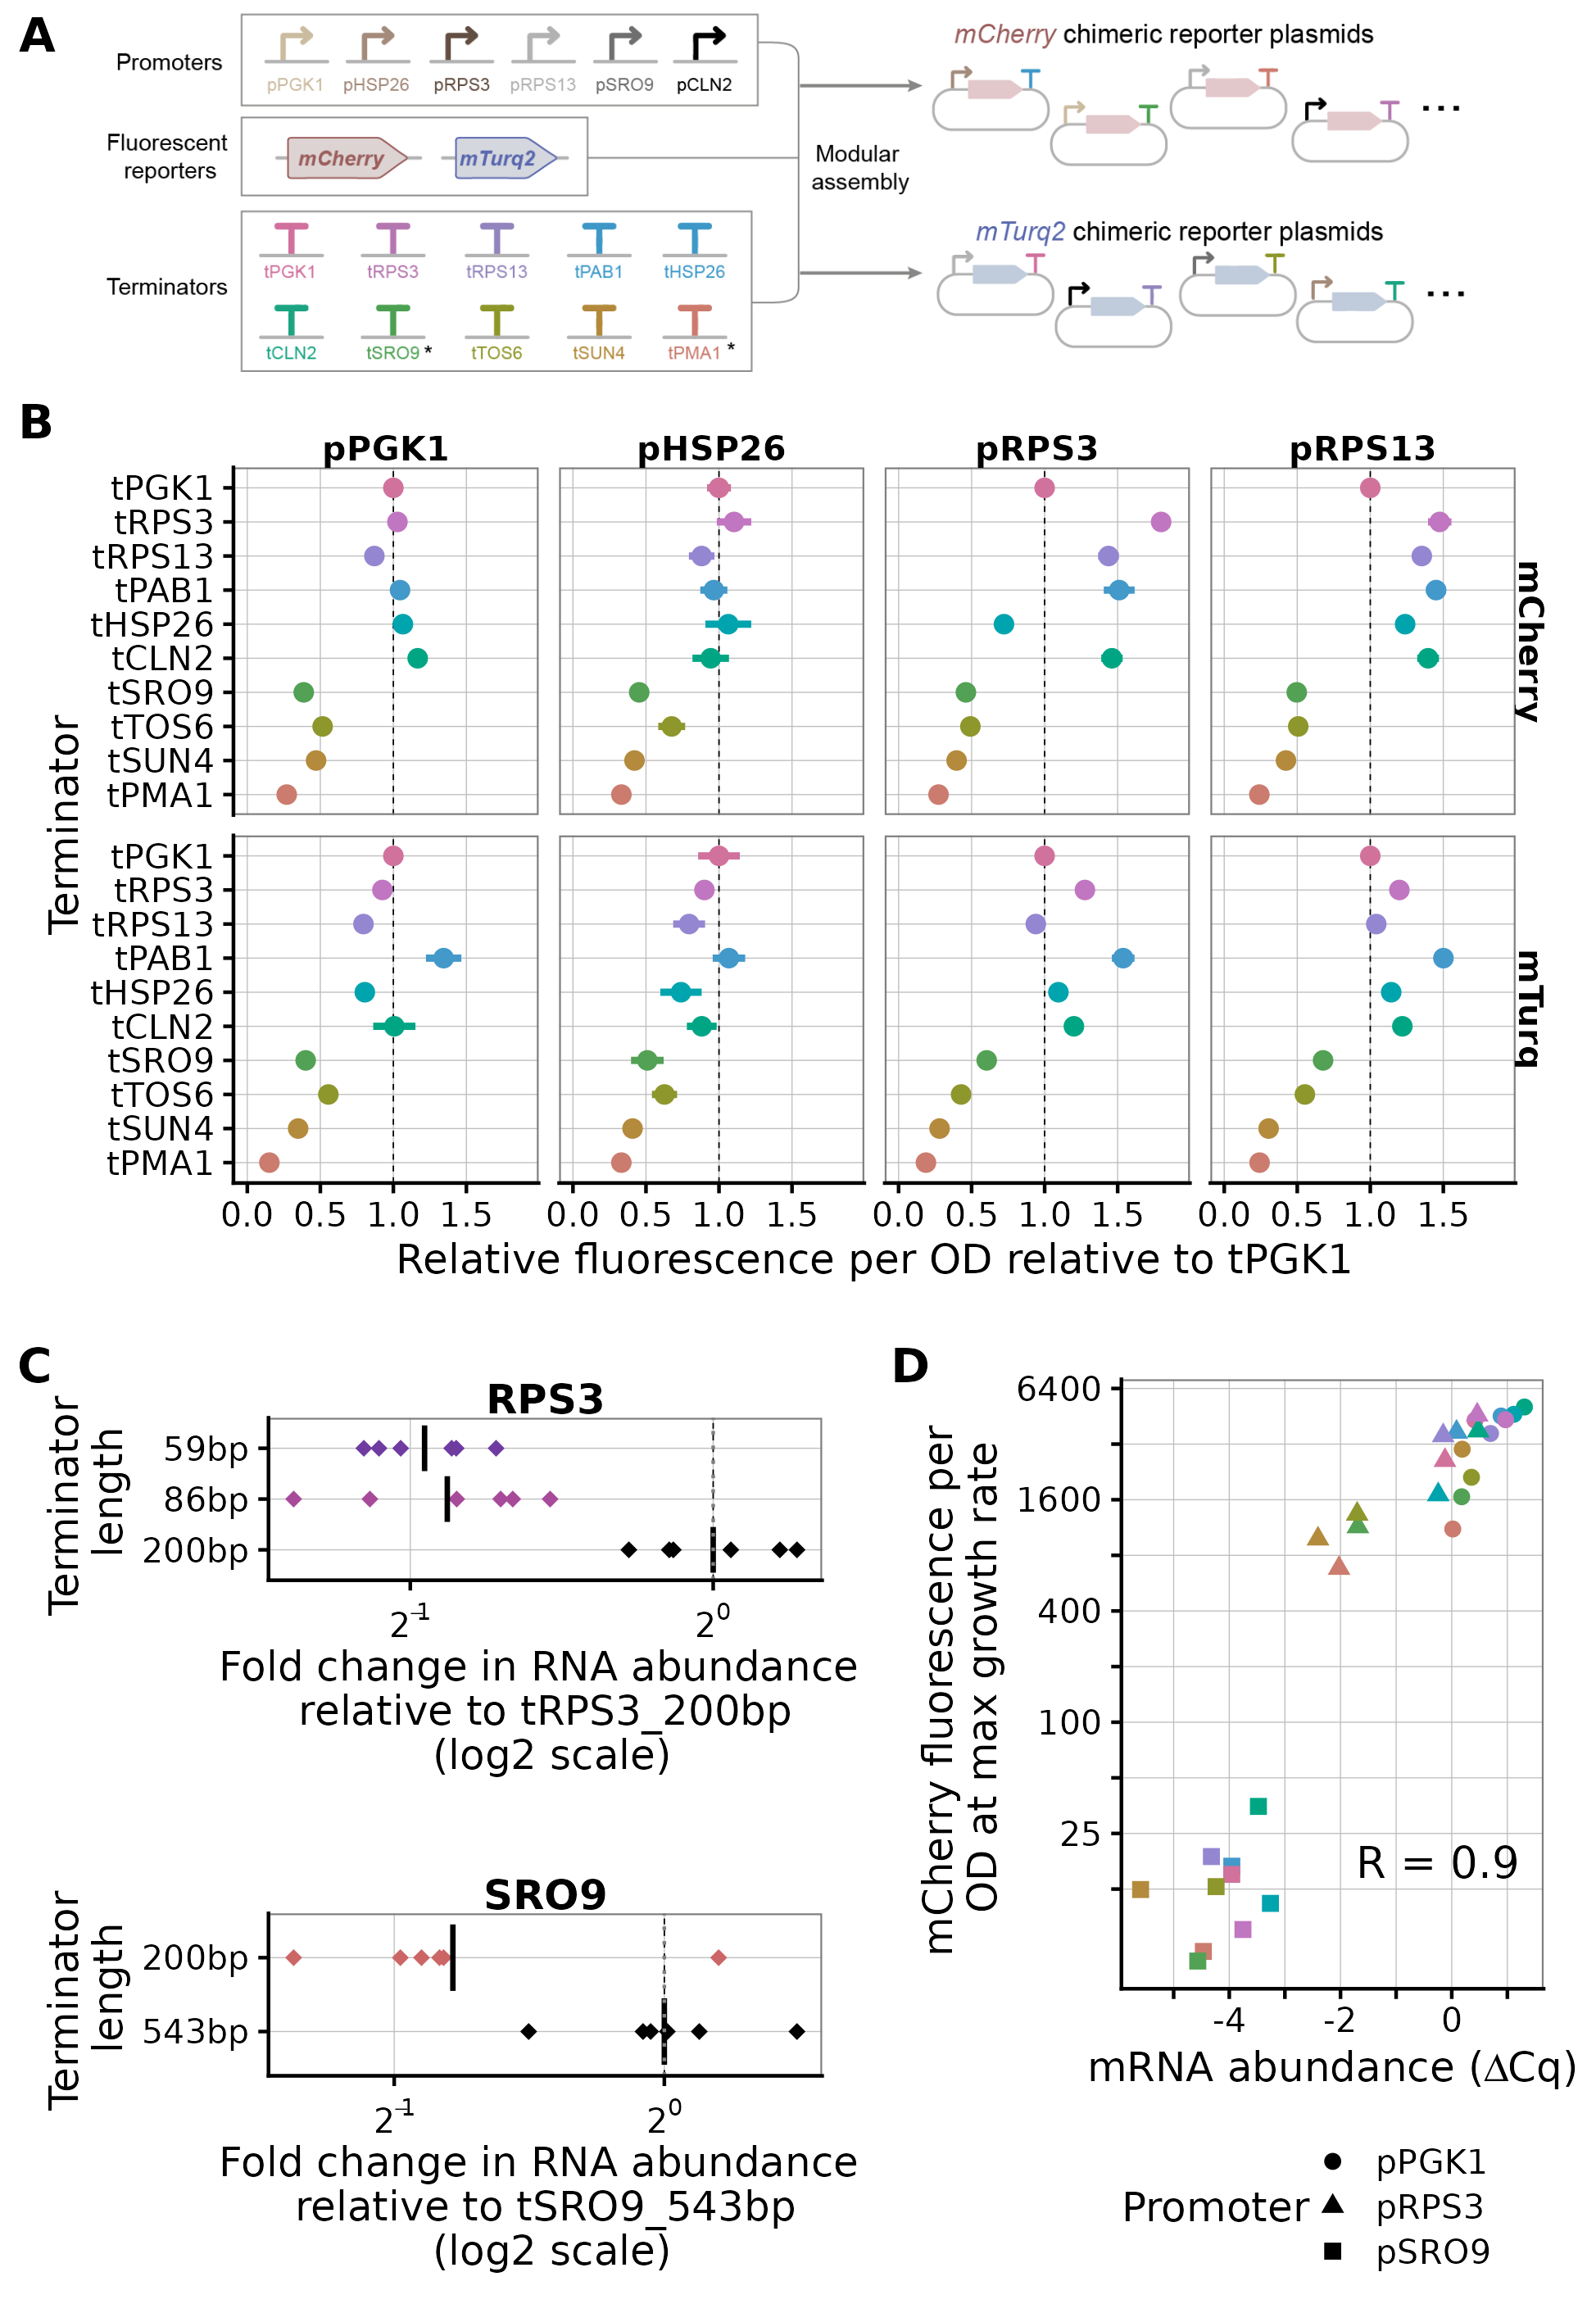
\includegraphics[width=0.8\linewidth]{pro_ter_swap_protein_and_norm_rna_exp_figure} 

}

\caption[Terminator contributions to gene expression are promoter, coding sequence and length dependent.]{\textbf{Terminator contributions to gene expression are promoter, coding sequence and length dependent.} (\textbf{A}) Design of chimeric reporter constructs with all combinations of 6 promoters, 2 fluorescent proteins, and 10 terminators, on a centromeric plasmid. Terminators highlighted with an asterisk have a terminator length longer than the library standard of 200bp because they have a median 3'UTR length greater than 200bp according to \parencite{Pelechano2013}. Panel created by Jamie Auxillos.  (\textbf{B}) Relative protein abundance from each terminator, normalized to a reference terminator tPGK1 for each matched promoter. The plot shows statistical summaries (mean and standard error) of at least 6 replicates for high-expression promoter data shown in Figure 1A. (\textbf{C}) RT-qPCR mRNA results targeting the mCherry ORF for pRPS3-mCherry-tRPS3 and pSRO9-mCherry-tSRO9 constructs with differing terminator lengths. (\textbf{D}) mCherry fluorescence correlates with RT-qPCR mRNA abundance for 3 promoters paired with all 10 terminators. Note that both axes use a \(log_2\) scale.}\label{fig:pro-ter-platereader-mCherry-mTurq-norm}
\end{figure}



\begin{table}

\centering
\fontsize{5}{7}\selectfont
\begin{tabular}[t]{>{\centering\arraybackslash}p{3em}|>{\centering\arraybackslash}p{6em}|>{\centering\arraybackslash}p{4em}|>{\centering\arraybackslash}p{6em}|>{\centering\arraybackslash}p{3em}|>{\centering\arraybackslash}p{6em}}
\hline
\begingroup\fontsize{7}{9}\selectfont \textbf{Gene Name}\endgroup & \begingroup\fontsize{7}{9}\selectfont \textbf{Systematic Name}\endgroup & \begingroup\fontsize{7}{9}\selectfont \textbf{Median 3’UTR Length}\endgroup & \begingroup\fontsize{7}{9}\selectfont \textbf{Construct Terminator Length}\endgroup & \begingroup\fontsize{7}{9}\selectfont \textbf{Usage}\endgroup & \begingroup\fontsize{7}{9}\selectfont \textbf{Function}\endgroup\\
\hline
PGK1 & YCR012W & 158 & 189 & S & Glycolysis\\
\hline
RPS3 & YNL178W & 86 & 200 & M\&S & Ribosomal\\
\hline
RPS13 & YDR064W & 92 & 200 & S & Ribosomal\\
\hline
PAB1 & YER165W & 150 & 200 & S & RNA Binding\\
\hline
HSP26 & YBR072W & 164 & 200 & S & Heat Shock\\
\hline
CLN2 & YPL256C & 203 & 200 & S & Cell Cyclin\\
\hline
SRO9 & YCL037C & 543 & 545 & S & RNA Binding\\
\hline
TOS6 & YNL300W & 256 & 256 & S & Cell Wall\\
\hline
SUN4 & YNL066W & 198 & 198 & S & Cell Wall\\
\hline
PMA1 & YGL008C & 421 & 421 & S & Transmembrane ATPase\\
\hline
TSA1 & YML028W & 112 & 219 & M & Redox Homestasis\\
\hline
PIR1 & YKL164C & 235 & 358 & M & Cell Wall\\
\hline
\end{tabular}
\caption[Summary of the terminator library.]{\label{tab:terminator-summary-table}\textbf{Summary of the terminator library.} The common gene name from which the terminator is extracted from is included alongside its systematic name. The median 3'UTR reported by \parencite{Pelechano2013} is a median over the lengths of each distinct isoform they detect. The usage of each motif is signified by S, for promoter-terminator swaps, or M, for motif insertion or deletion. A short summary of the protein function is included.}
\end{table}

Measuring fluorescence with a plate reader showed that, as expected, promoter choice dominated overall protein output.
We observed up to 100-fold changes in fluorescence between the 4 highest expressing promoters (Supplementary Figure \ref{fig:raw-pro-ter-swap-protein-fluo}A) and the 2 lowest expressing promoters (Supplementary Figure \ref{fig:raw-pro-ter-swap-protein-fluo}B; mCherry log2 fold change = 7.33, p.value = 0.000).
Expression from the stress-induced pHSP26 was notably more variable than from pPGK1 and pRPS's, across biological replicates, when combined with both coding sequences and a variety of terminators.
We also confirmed that most differences in protein outputs are accounted for by changes in mRNA abundance by checking a subset of mCherry constructs using RT-qPCR (\(R = 0.888\), Figure \ref{fig:pro-ter-platereader-mCherry-mTurq-norm}D).

Terminators also affect protein output with 5-fold changes in fluorescence seen within the same promoter-CDS sets (pPGK1-mTurq-tPMA1 log2 fold change = -2.73, p.value =\(1.19 \times 10^{-41}\)), relative to the tPGK1 terminator of each group (Figure \ref{fig:pro-ter-platereader-mCherry-mTurq-norm}B, Supplementary Table \ref{tab:norm-terminator-sig-effect}).
We focus on constructs with high-expression promoters due to the poor signal to noise ratio at low expression levels.
The interaction of coding sequence and terminator is seen most clearly for tPAB1.
tPAB1 is consistently the most highly expressed terminator in mTurquoise2 constructs, but is more variable in mCherry constructs.
Meanwhile, tPGK1 highlights the interactions of promoter and terminator.
tPGK1 is one of the most highly expressing terminators when paired with pPGK1 and pHSP26, but is up to 40\% lower in expression when paired with pRPS3 or pRPS13.
Overall, our results show that the contributions of terminators (including 3'UTRs) to gene expression depend on other parts within the gene.

We further investigated the effects of terminators on mRNA levels by comparing constructs with extended vs truncated terminators.
It is known that disrupting the transcription termination signal lowers expression (10, 46).
However, standardised parts libraries often assume a fixed terminator length for all genes, which is likely to omit the termination signal for genes with longer terminators.
In the case of the YeastFab parts library \parencite{Guo2015} the fixed terminator length is 200bp.
We compared a gene with a median 3'UTR length less than 200bp, RPS3 to a gene with a median 3'UTR length greater than 200bp, SRO9.
The median length of the native RPS3 3'UTR is 86nt \parencite{Pelechano2013}; truncating the terminator to 86bp or 59bp reduces transcript protein output by almost 2-fold (86bp Fold Change = 0.544, p-value = \(2.6 \times 10^{-4}\); 59bp Fold Change = 0.517, p-value = \(7.8 \times 10^{-6}\); Figure \ref{fig:pro-ter-platereader-mCherry-mTurq-norm}C).
The median length of the native SRO9 3'UTR is 543nt \parencite{Pelechano2013}; extending the terminator length to 543bp increases transcript protein output by almost 2-fold (Fold Change = 0.581, p-value = 0.01; Figure \ref{fig:pro-ter-platereader-mCherry-mTurq-norm}C).
This validates our assay's ability to detect known regulatory signals affecting transcription termination, while highlighting the importance of using well-informed annotations to construct parts libraries for synthetic biology.
Note that we used the longer 543bp SRO9 terminator, and a similarly extended 421bp PMA1 terminator, for the main set of constructs (Figure \ref{fig:pro-ter-platereader-mCherry-mTurq-norm}).

\subsection{Candidate cis-regulatory elements contribute to transcript decay rates}

Next, we investigated how the regulatory effects of CREs contained within terminator regions depend on their context.
First, 69 suitable CREs to test for context dependence were found through a literature search.
All were suspected sequence motifs for mRNA binding proteins, several directly associated with proteins involved in mRNA degradation (3, 12, 13).
Any motifs that were found in fewer than 6 gene 3'UTRs, as annotated by \parencite{Pelechano2013}, were removed.

We quantified the regulatory effects of the remaining 38 candidate motifs by applying a linear model predicting half-life to 2 recent transcriptome-wide analyses of mRNA decay that used metabolic labeling (41, 49).
These datasets are loosely correlated in their half-life measurements across 4188 genes reported in both datasets, \(R = 0.63\) (Figure \ref{fig:hlife-decay-model}A). However, \parencite{Chan2018} estimated substantially smaller half-lives.
\parencite{Chan2018} also had greater coverage of genes in the yeast genome, 5529 vs 4304, and used multiple time points to determine half-lives.
Following (13), we constructed a linear model to predict a transcript's half-life using the counts of motifs in its 3'UTR, the length of the 3'UTR, and the relative codon usage in each transcript's coding sequence (see Material and Methods).
The linear model performed similarly on both datasets by explaining 44\% and 41\% of the variability in half-lives for the \parencite{Chan2018} and \parencite{Sun2013} datasets respectively (Figure \ref{fig:hlife-decay-model}C).
This predictive power is comparable to the squared correlation between the datasets (\(R^2 = 0.40\)).
Motifs that did not significantly contribute to the model were automatically filtered out using a greedy algorithm maximising the Akaike information criterion (AIC) during both training stages.
Approximately 1.7\% of the variance is explained by 7 significant motifs, with 42.0\% explained by codon usage (Supplementary Table \ref{tab:hlife-variance-table}), consistent with previous analyses (13, 50).
The top 7 most significant motifs from the \parencite{Chan2018} data showed similar regulatory behaviour when tested on their own in the \parencite{Sun2013} data, except for TGTAAATA which was stabilising in one dataset and destabilising in another, as we later discuss (Figure \ref{fig:hlife-decay-model}B).

We selected 4 motifs for exploring context dependence: TGTAHMNTA, GTATACCTA, HWNCATTWY, and ATATTC (Table \ref{tab:motif-summary-table}).
TGTAHMNTA and GTATACCTA were chosen as they had the largest coefficients amongst significant decay and stability motifs, respectively.
HWNCATTWY was chosen due to its statistically significant effect in both datasets and, as it co-occurs with TGTAHMNTA in 68 native 3'UTRs, because it could be used for testing motif interactions.
The final selected motif was ATATTC, as it is a statistically significant decay motif in both datasets, and it has been previously shown to lower mRNA abundance when inserted in reporter constructs (13).
Functionally, TGTAHMNTA is the binding motif for Puf4p, and HWNCATTWY is associated with Khd1p/Hek2p-bound transcripts \parencite{Hogan2008}.
However, it is not known how ATATTC and GTATACCTA affect mRNA decay.



\begin{table}

\centering
\begingroup
\setlength{\tabcolsep}{5pt}
\fontsize{7}{9}\selectfont
\begin{tabular}[t]{>{\centering\arraybackslash}p{6em}|>{\centering\arraybackslash}p{5.2em}|>{\centering\arraybackslash}p{5.5em}|>{\centering\arraybackslash}p{3.5em}|>{\centering\arraybackslash}p{2.6em}|>{\centering\arraybackslash}p{4em}|>{\centering\arraybackslash}p{2.6em}|>{\centering\arraybackslash}p{4em}|>{\centering\arraybackslash}p{4em}}
\hline
\textbf{Consensus Seq} & \textbf{Inserted Motif} & \textbf{Deleted Motif} & \textbf{Source} & \textbf{Chan Coef} & \textbf{Chan p.value} & \textbf{Sun Coef} & \textbf{Sun p.value} & \textbf{Notes}\\
\hline
GTATACCTA & GTATACCTA & GTATACCTA & Shalgi & 0.500 & 1.9e-02 & 0.280 & 0.3300 & Unknown\\
\hline
ATATTC & ATATTC & ATATTC & Cheng & -0.075 & 1.4e-03 & -0.170 & 0.0000 & Decay motif\\
\hline
HWNCATTWY & TTTCATTTC & CTTCATTTC ATACATTAT AATCATTAT & Hogan & -0.084 & 4.9e-06 & -0.061 & 0.0026 & Khd1/Hek2 associated motif\\
\hline
TGTAHMNTA & TGTACAATA & TGTACATTA & Hogan & -0.230 & 0.0e+00 & -0.056 & 0.1800 & Puf4p binding motif\\
\hline
\end{tabular}
\endgroup
\caption[Summary of shortlisted motif characteristics.]{\label{tab:motif-summary-table}\textbf{Summary of shortlisted motif characteristics.} The first 3 columns hold the consensus sequence for each motif and the exact versions deleted from or inserted into the host terminators. Then, we report the paper from which the motif was selected from; \parencite{Hogan2008}, \parencite{Cheng2017} or \parencite{Shalgi2005}. Next, each motif's coefficient given by the linear model predicting either the \parencite{Chan2018} or the \parencite{Sun2013} half-life datasets are included. Finally, the table includes notes on motif functions.}
\end{table}



\begin{figure}[p]

{\centering 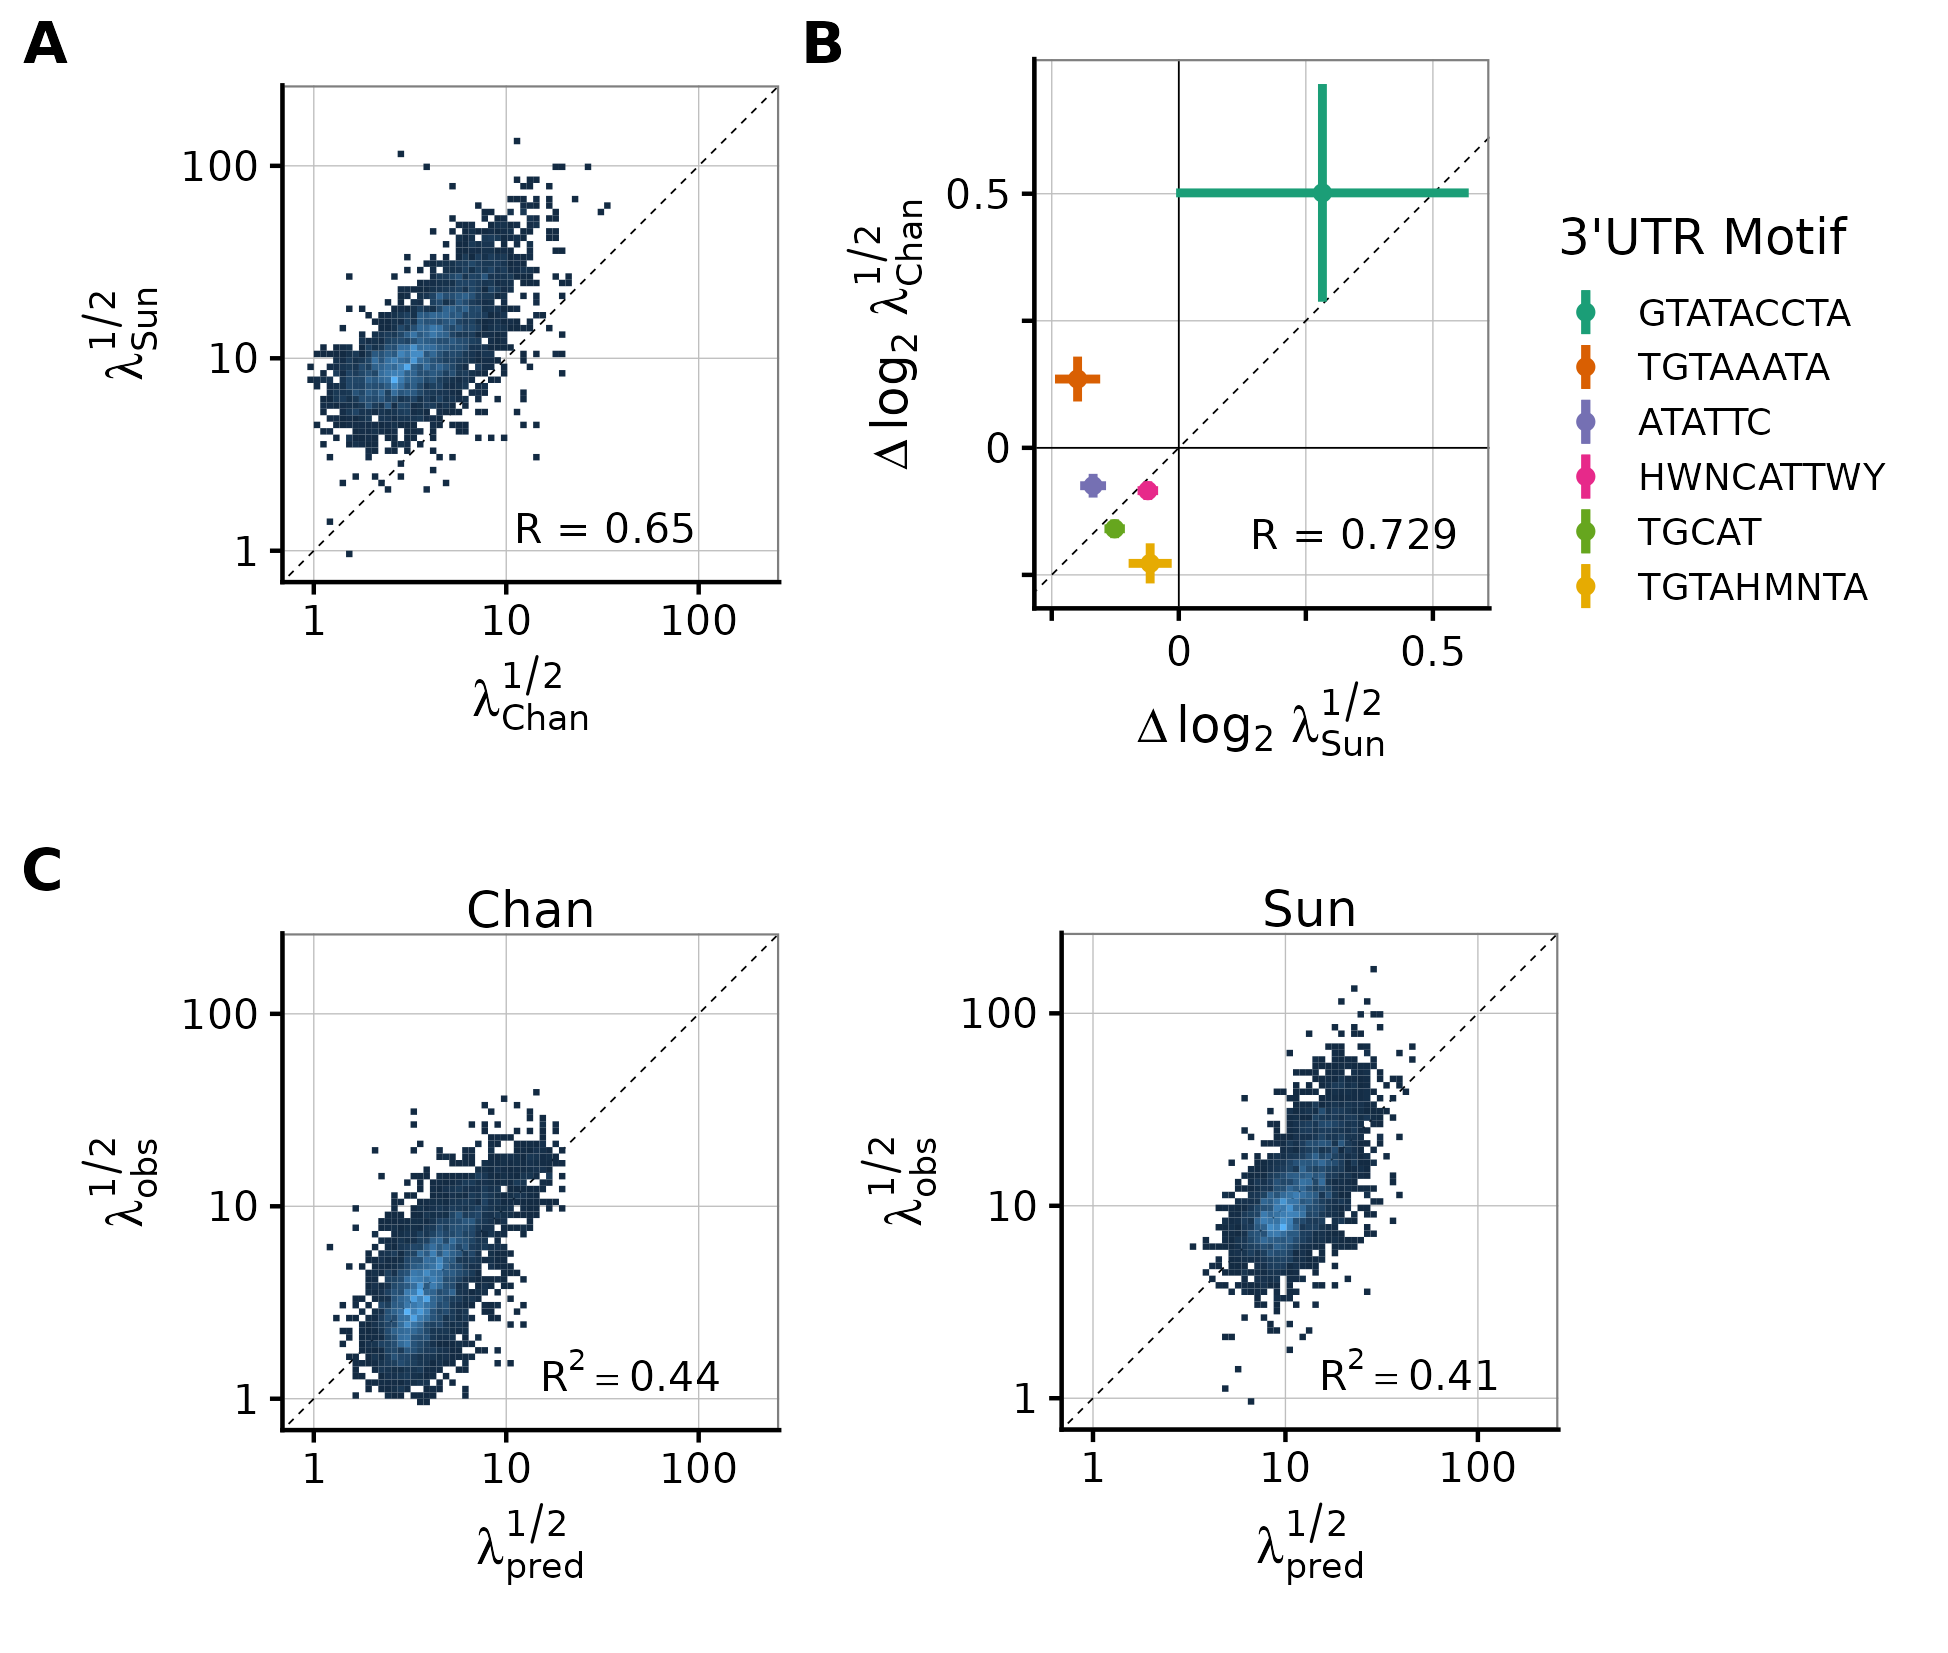
\includegraphics[width=0.98\linewidth]{hlife_model_multi_fig} 

}

\caption[A linear model of transcript half-life quantifies the effect of candidate terminator motifs on half-life.]{\textbf{A linear model of transcript half-life quantifies the effect of candidate terminator motifs on half-life.} (\textbf{A}) Correlation between the 2 transcript half-lives (\(\lambda\)), in minutes, reported in the \parencite{Chan2018} and \parencite{Sun2013} datasets. (\textbf{B}) Predicted contributions to log2 half-life for chosen motifs in the \parencite{Chan2018} and \parencite{Sun2013} datasets. (\textbf{C}) Predicted vs actual transcript half-lives calculated by a linear model of codon and motif usage trained on the \parencite{Chan2018} and \parencite{Sun2013} datasets.}\label{fig:hlife-decay-model}
\end{figure}

\subsection{Quantification of differential expression due to motif insertion or mutagenesis in multiple 3'UTRs}

To quantify the effects and composability of selected motifs in different contexts, we designed a further set of reporter constructs (Figure \ref{fig:tRPS3-tTSA1-design-and-qpcr}A).
We first chose the ribosomal protein terminator tRPS3, as it was the only terminator in our initial library that did not contain any of the selected motifs.
We selected thioredoxin peroxidase tTSA1 as the second host terminator because it also lacks selected motifs and has similar length to tRPS3.
In each host terminator we chose 3 motif insertion sites, selecting for: minimum impact on transcript secondary structure, avoiding known transcription termination elements, and matching the positions of motifs in native genes.
Having 3 insertion sites enabled us to quantify combinations of motifs, including duplicates of weaker motifs to increase the likelihood of detecting a clear effect on gene expression.
We chose TGTACAATA and TTTCATTTC sequences as explicit versions of the TGTAHMNTA and HWNCATTWY consensus motifs respectively, and checked that these explicit versions have similar predicted effects on half-life transcriptome-wide (Supplementary Tables \ref{tab:HWNCATTWY-motif-coef}, \ref{tab:TGTAHMNTA-motif-coef}).
Altogether, 7 variant terminators were designed for these 2 host terminators: the wildtype terminator, a control to test the insertion sites with randomly generated sequences, 4 testing the effects of inserting each motif individually and a final variant to test interactions between the TGTAHMNTA and HWNCATTWY motifs.
We created a construct library by pairing each terminator with three different promoters; its native promoter pairing (pRPS3 or pTSA1), the high-expression promoter pPGK1, and the low-expression promoter pSRO9.

Motifs predicted to affect half-life affect mRNA abundance when inserted into tRPS3 in reporter constructs (Figure \ref{fig:tRPS3-tTSA1-design-and-qpcr}B).
We measured mRNA abundance by RT-qPCR across 6 biological replicates, each quantified in 3 technical replicates and normalised by the \(\Delta Cq\) method against values from 3 reference mRNAs (see methods).
Insertion of 2 copies of ATATTC (mod\_NAA) generally lowers the mRNA abundance, as much as 4-fold when paired with the pRPS3 promoter.
Insertion of either TGTAHMNTA (mod\_NTN), or 2 copies of HWNCATTWY (mod\_HNH), tends to decrease mRNA abundance, and their combined insertion (mod\_HTH) tends to decrease mRNA abundance even further.
The putative stability motif GTATACCTA (mod\_NGG) does not consistently or strongly affect mRNA abundance.
However, comparison of the WT and control (mod\_NNN) terminators does show that the creation of the insertion sites alone has an effect on mRNA levels (Supplementary Table \ref{tab:insertion-construct-ttest}).

Inserting the same motifs into our second host terminator gives qualitatively similar results (Figure \ref{fig:tRPS3-tTSA1-design-and-qpcr}C).
Decay motifs generally lead to decay, although ATATTC (mod\_NAA) has a weaker effect in tTSA1 than in tRPS3, and TGTAHMNTA (mod\_NTN) has a stronger effect in tTSA1 than tRPS3.
The putative stability motif GTATACCTA (mod\_NGG) again has little effect.

We next quantified the effects of removing decay motifs from a native yeast terminator.
We selected the cell wall protein PIR1 as our host terminator as it is only 258 bp \parencite{Pelechano2013} and a \emph{de-novo}-synthesizable terminator that contains the ATATTC, TGTAHMNTA, and HWNCATTWY motifs.
We designed 8 terminators in which the motif occurrences in tPIR1 were replaced by scrambled sequences (Figure \ref{fig:tPIR1-design-and-qpcr}A).
We found that the removal of almost any decay motif from tPIR1 results in an increase in mRNA levels (Figure \ref{fig:tPIR1-design-and-qpcr}B; Supplementary Table \ref{tab:deletion-construct-ttest}).

We confirmed that motif-dependent changes in mRNA abundance are reflected in protein abundance by measuring the fluorescence from a subset of reporter constructs with native promoter-terminator pairings (Supplementary Figure \ref{fig:protein-vs-RNA-plot-motifs}).
The high correlation (\(R = 0.96, 0.68, 0.86\) for tRPS3, tTSA1, tPIR1 constructs respectively) demonstrates that these combinations of decay motifs that change mRNA abundance also change the protein output, as expected.

Comparison of mRNA abundance across all constructs (Figure \ref{fig:tRPS3-tTSA1-design-and-qpcr}B, \ref{fig:tRPS3-tTSA1-design-and-qpcr}C, \ref{fig:tPIR1-design-and-qpcr}B) shows motif contributions change in magnitude but not direction depending on the context of the rest of the construct.
The insertion of almost any decay motif into tTSA1 or tRPS3 results in a decrease in mRNA abundance, and removal of these from from tPIR1 results in an increase in mRNA abundance.
However, the quantitative effects vary depending both on the immediate motif context in the host terminator and on the more distant context given by the promoter.

\begin{figure}[p]

{\centering 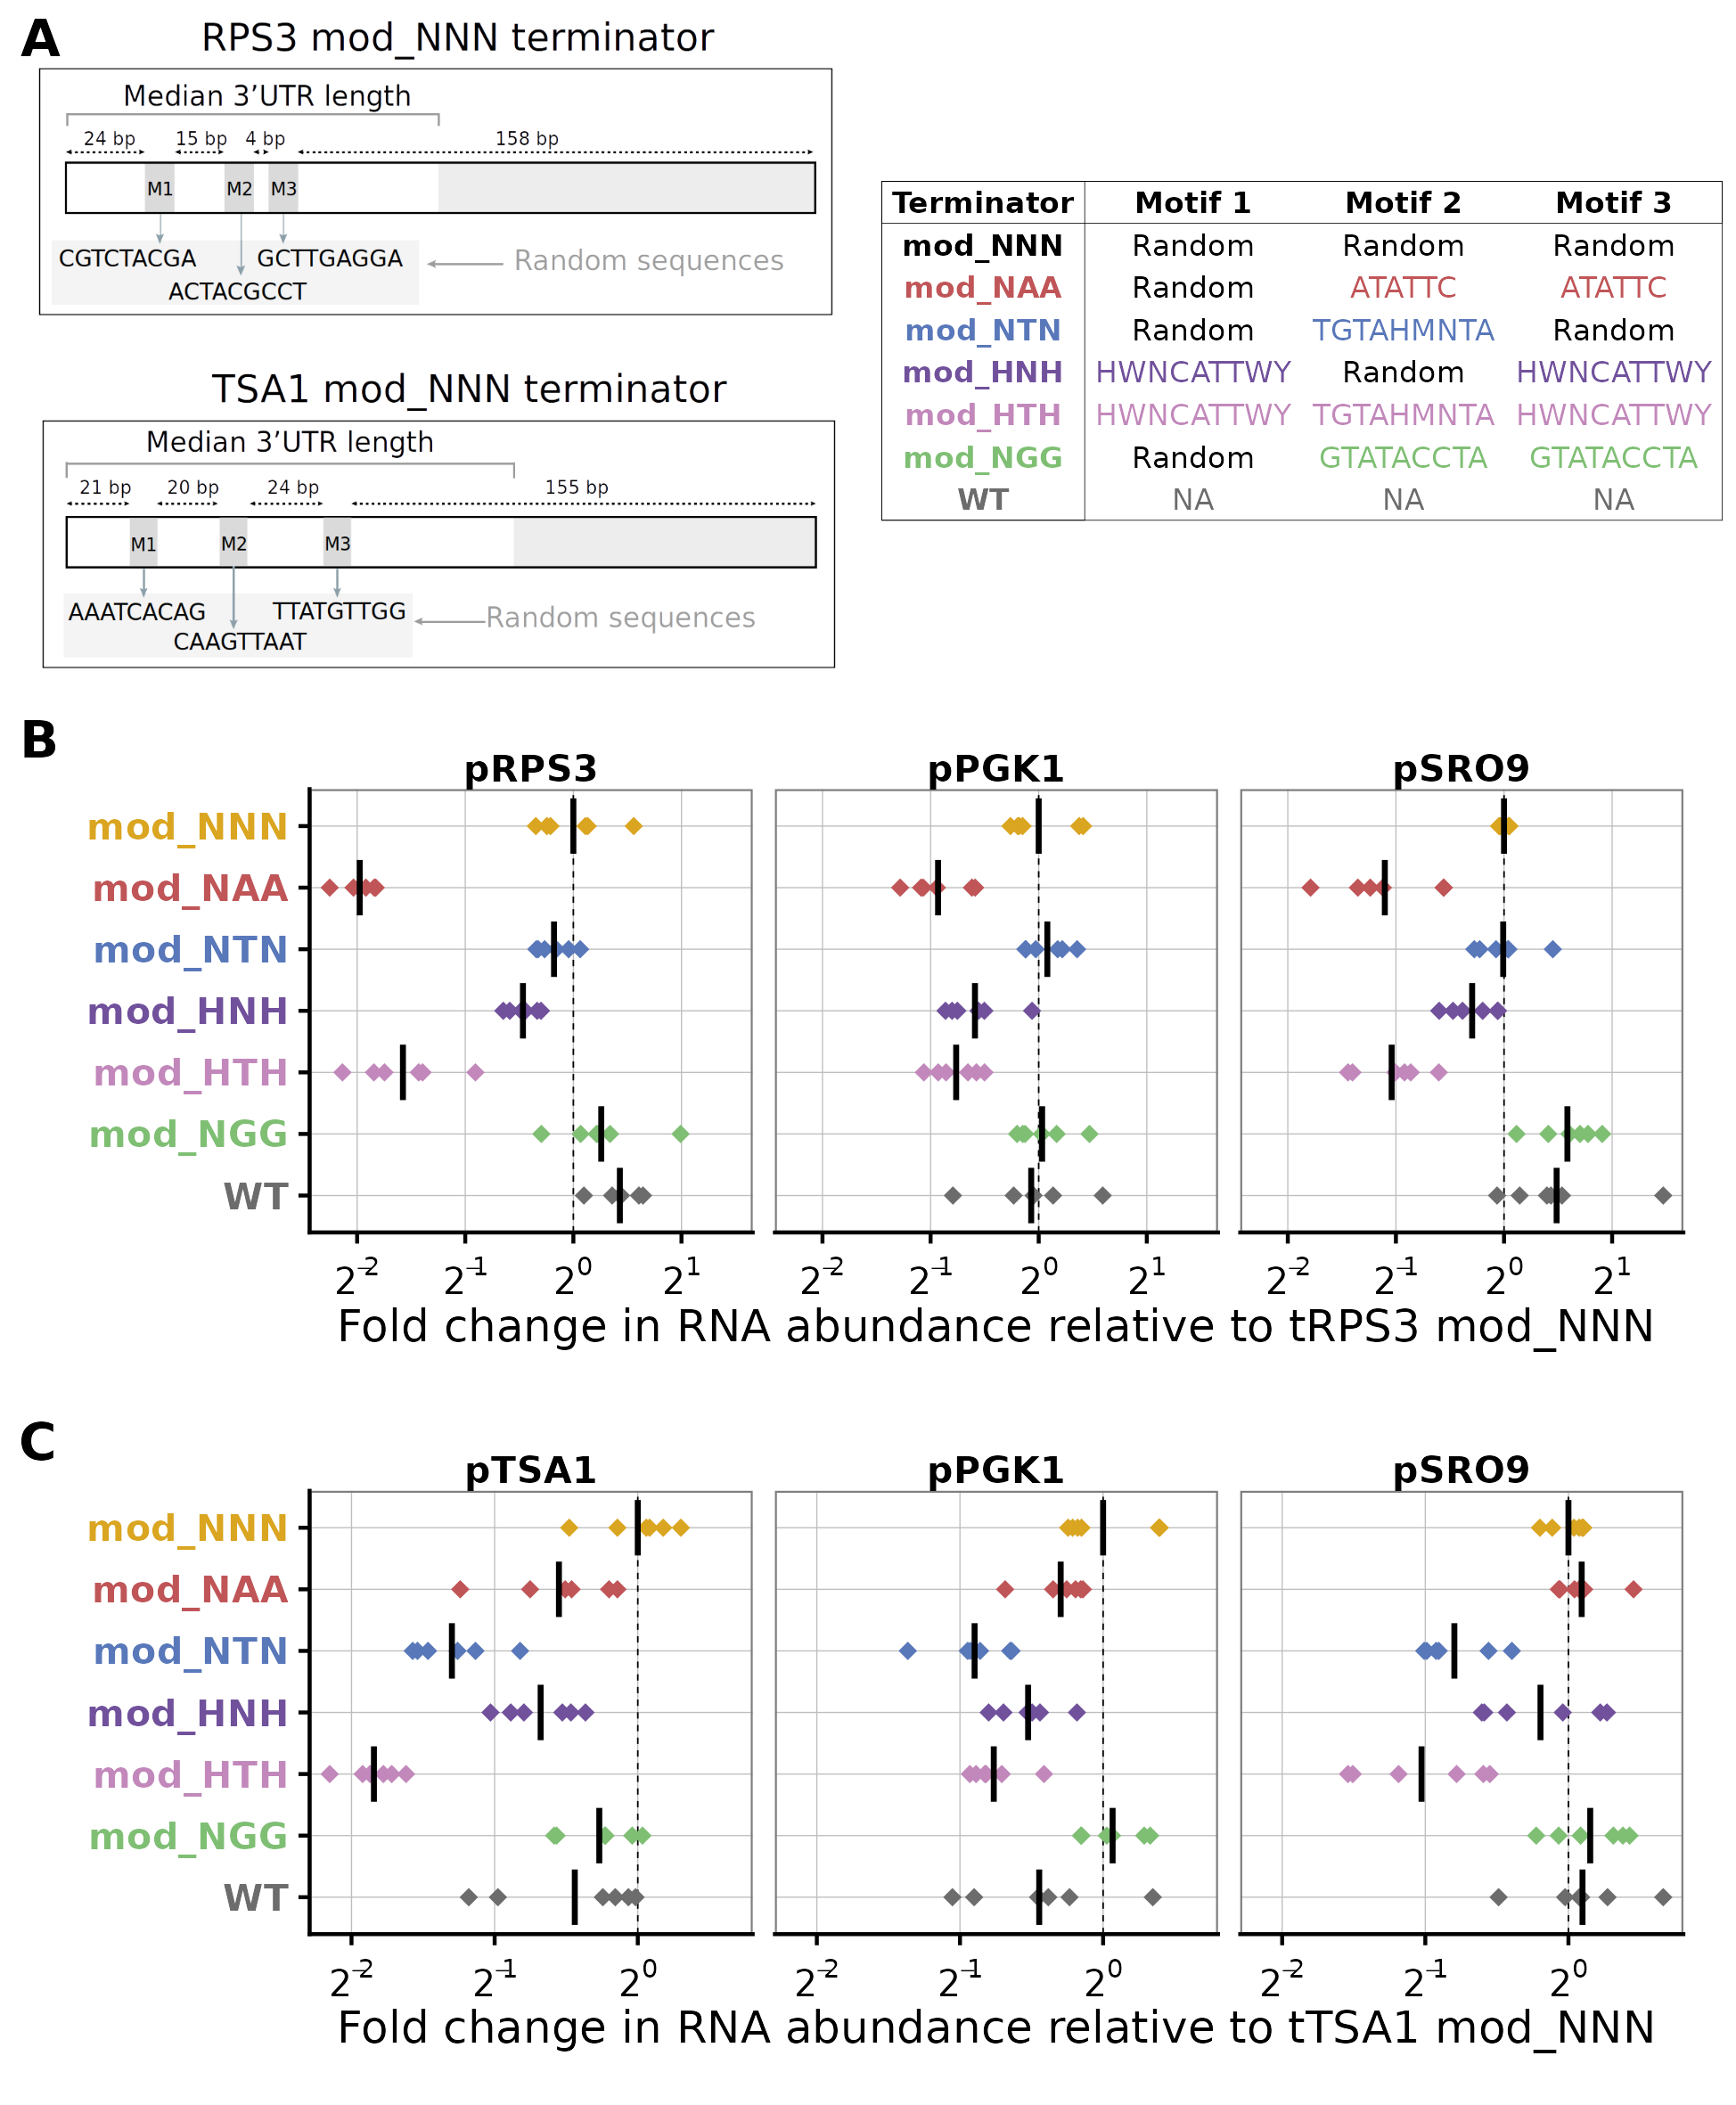
\includegraphics[width=0.98\linewidth]{insertion_constructs_design_and_qpcr} 

}

\caption[Motifs inserted into RPS3 and TSA1 host terminators change transcript abundance in RT-qPCR measurements.]{\textbf{Motifs inserted into RPS3 and TSA1 host terminators change transcript abundance in RT-qPCR measurements.} (\textbf{A}) Design of motif insertion sites in native RPS3 and TSA1 terminators, highlighting random insertion used as a negative control. Panel created by Jamie Auxillos. (\textbf{B}) Fold changes in transcript abundance for tRPS3 constructs paired with 3 promoters: pRPS3, pPGK1 and pSRO9. (\textbf{C}) Fold changes in transcript abundance for tTSA1 constructs paired with three promoters: pTSA1, pPGK1 and pSRO9. Each diamond represents a biological replicate, averaged over 3 technical replicates. The vertical line represents the mean of all 6 biological replicates. Fold changes are relative to the abundance of the mod\_NNN construct, i.e. $2^{\Delta\Delta Cq}$ (see methods).}\label{fig:tRPS3-tTSA1-design-and-qpcr}
\end{figure}

\begin{figure}[p]

{\centering 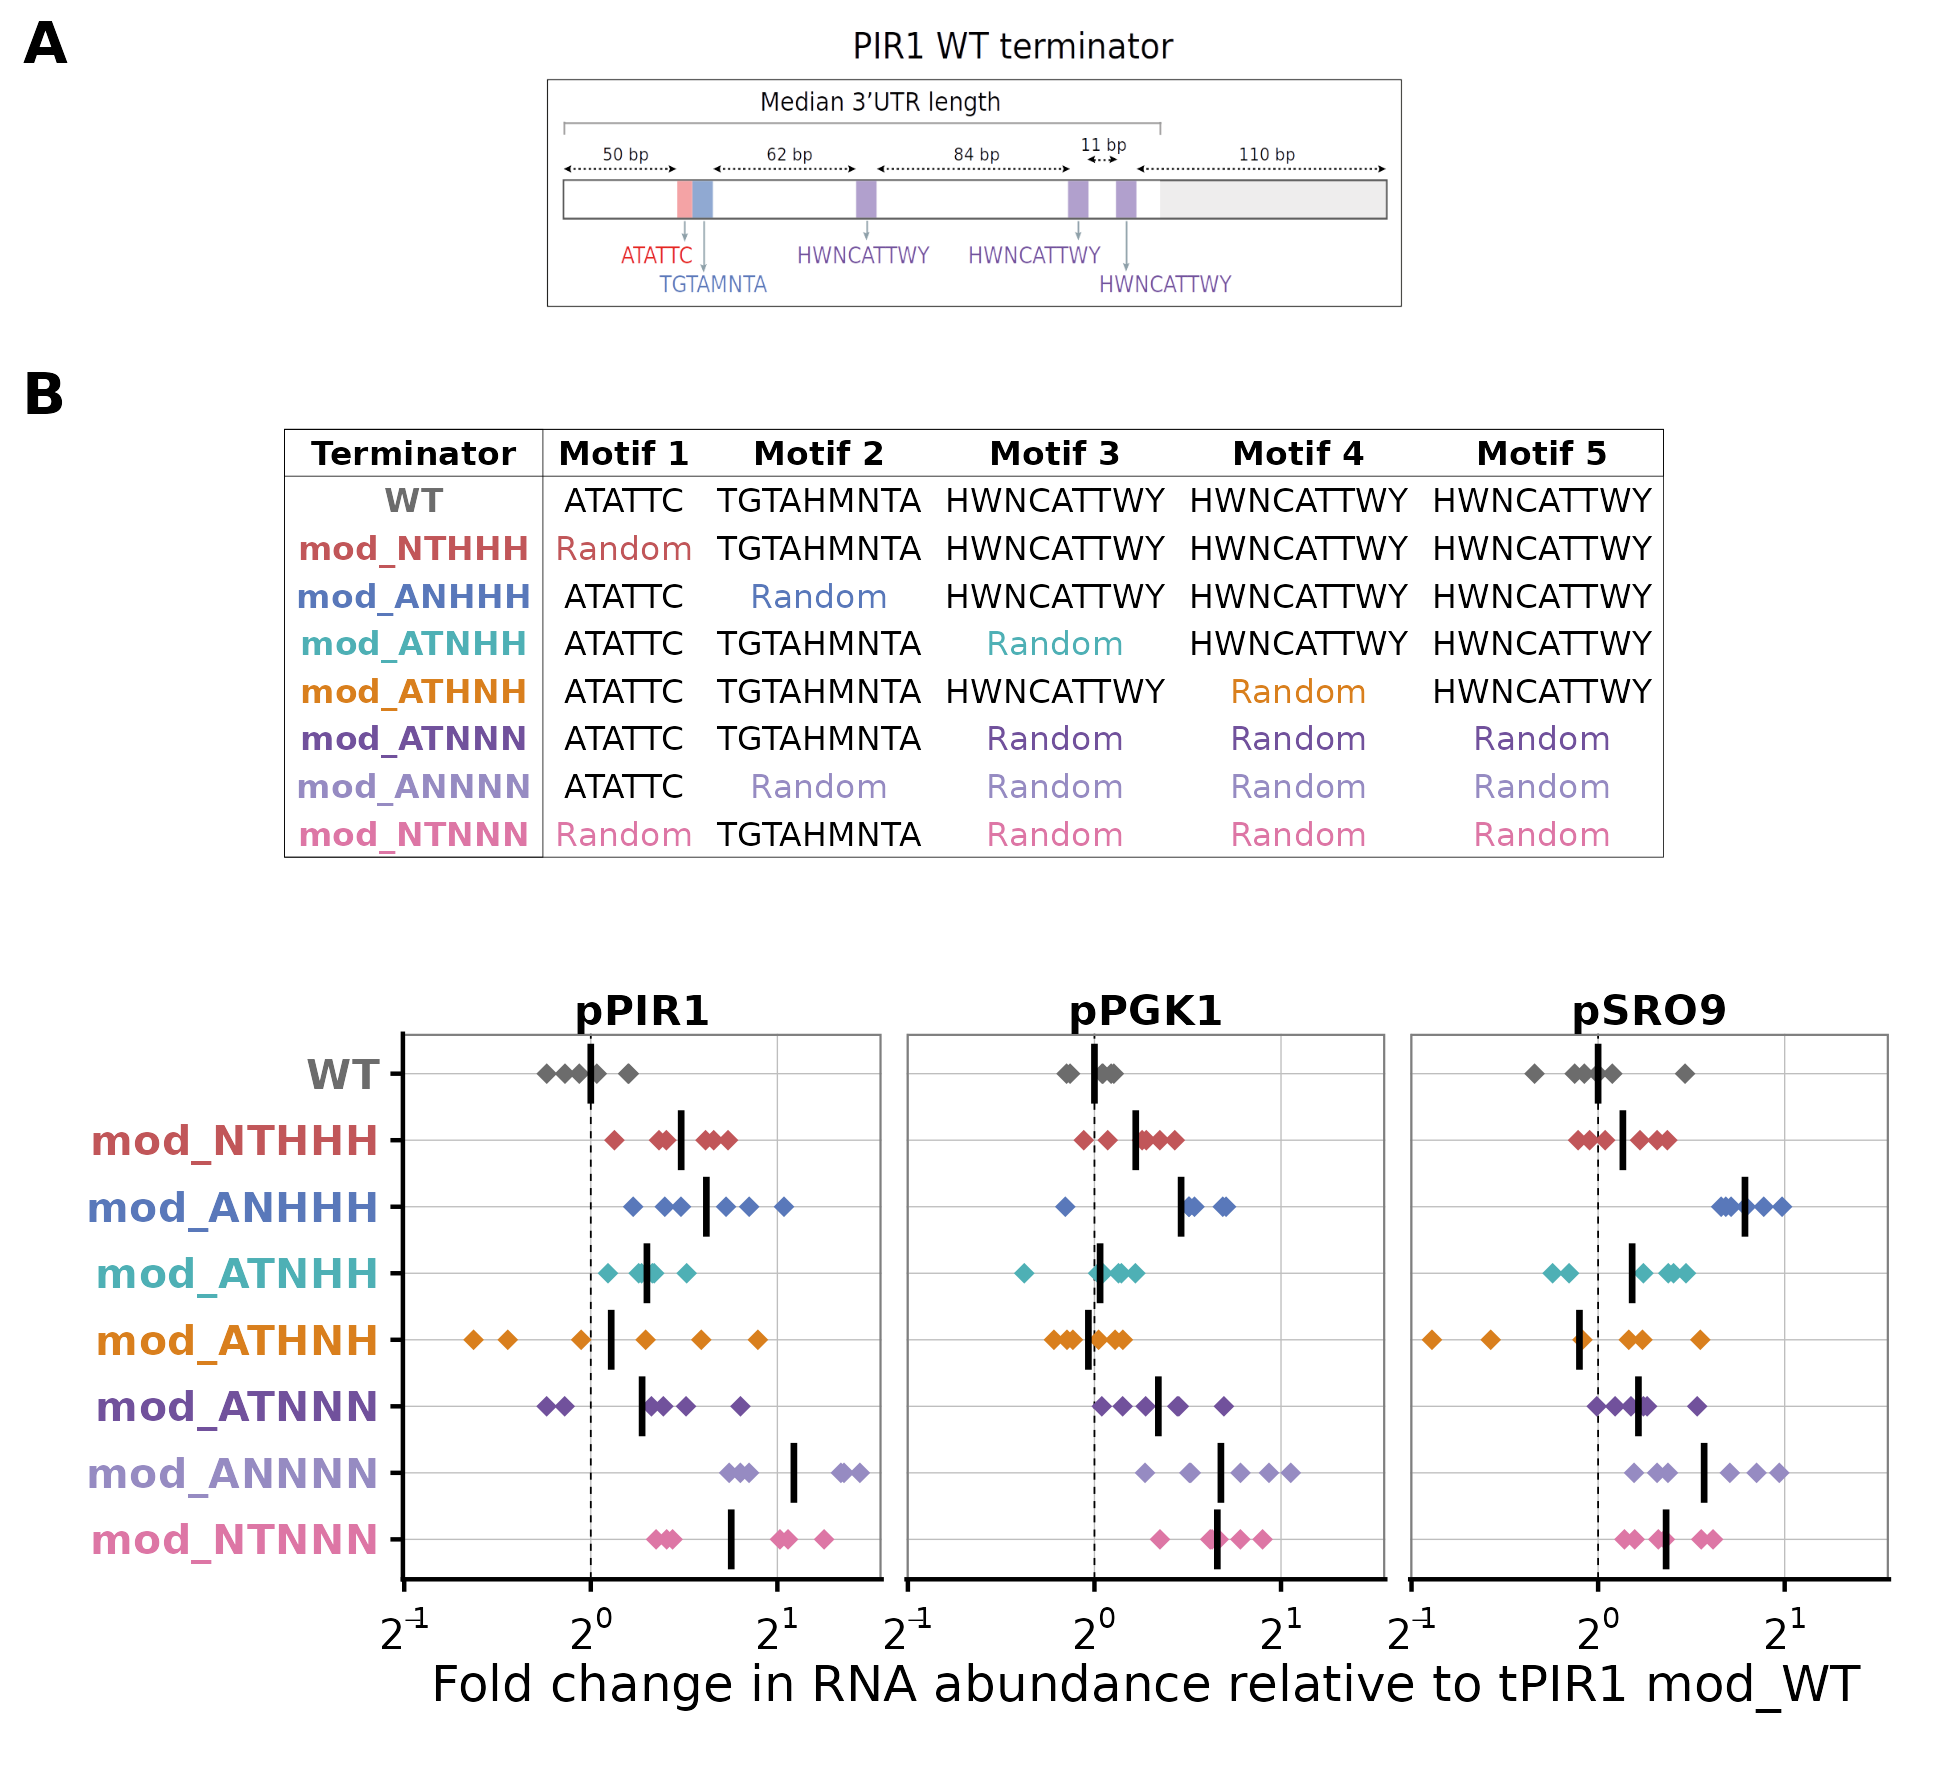
\includegraphics[width=0.98\linewidth]{tPIR1_design_and_qpcr.png} 

}

\caption[Motifs removed from PIR1 host terminators change transcript abundance in RT-qPCR measurements.]{\textbf{Motifs removed from PIR1 host terminators change transcript abundance in RT-qPCR measurements.} (\textbf{A}) Design of PIR1 constructs with combinations of motifs replaced by random nucleotide sequences. Panel created by Jamie Auxillos. (\textbf{B}) Fold changes in transcript abundance for tPIR1 constructs paired with 3 promoters: pPIR1, pPGK1 and pSRO9. Each diamond represents a biological replicate, averaged over 3 technical replicates. The vertical line represents the mean of all 6 biological replicates. Fold changes are relative to the abundance of the WT construct, i.e. $2^{\Delta\Delta Cq}$ (see methods).}\label{fig:tPIR1-design-and-qpcr}
\end{figure}

\subsection{Motif effects on gene expression depend both on terminator context and promoter pairing}

We compared the effects of cis-regulatory motifs on mRNA abundance to predicted effects inferred from the transcriptome-wide measurements of half-life.
First, we trained a linear model using the RT-qPCR results to estimate the change in log2 mRNA abundance (i.e.~\(\Delta Cq\)) due to the presence of a motif in each promoter and terminator combination.
Using a simple model of transcript production and decay, we can argue that changes in mRNA abundance are directly proportional to changes in mRNA half-life (see methods).
Therefore, we compared the motif's estimated change in log2 mRNA abundance to that predicted due to changes in log2 half-life, estimated from our transcriptome-wide analysis of the \parencite{Chan2018} dataset.
The effect of motifs in reporter constructs is correlated with the predictive model, but the strength of the correlation depends on context (Figure \ref{fig:hlife-predict-vs-abundance-and-motif-context-dependence}A).
Constructs with inserted motifs (i.e.~tRPS3 and tTSA1 constructs) had a lower correlation with predicted effects than constructs with deleted motifs (i.e.~tPIR1 constructs).
Interestingly, motif effects on mRNA abundance appear to be greater than that predicted from their effect on half-life when their host terminator is paired with its native promoter.

We next directly compared the estimated coefficients for each motif's effect on mRNA abundance across promoter-terminator pairing (Figure \ref{fig:hlife-predict-vs-abundance-and-motif-context-dependence}B).
The effect of a motif depends on terminator context.
For example, ATATTCA reduces mRNA abundance substantially more when inserted in tRPS3 than in tTSA1 (pRPS3-tRPS3 log2 Fold Change = -0.99, p-value = \(1.5 \times 10^{-13}\); pTSA1-tTSA1 log2 Fold Change = -0.26, p-value = \(7.3 \times10^{-3}\)).
Meanwhile, TGTAHMNTA significantly reduces mRNA abundance when inserted in tTSA1, but not tRPS3, whichever promoter is chosen (pRPS3-tRPS3 log2 fold Change = -0.18, p-value = 0.37; pTSA1-tTSA1 log2 fold Change = -1.30, p-value = \(1.0 \times10^{-7}\)).
Promoter choice also influences the magnitude of a motif's contribution to mRNA levels.
For the ATATTC, TGTAHMNTA and HWNCATTWY motifs the greatest reduction in mRNA abundance occurred when native promoter-terminator pairings are measured.
This is true for all 3 decay motifs across all 3 host terminators, except for HWNCATTWY in pRPS3-tRPS3 constructs (Supplementary Table \ref{tab:motif-abundance-effect-table}).

Regulatory interactions between different motifs also change depending on host terminator and promoter context.
We included an interaction term that quantifies how the effect of including both HWNCATTWY and TGTAHMNTA together differs from the sum of the effects of including these motifs individually.
The combination of TGTAHMNTA and HWNCATTWY in tRPS3 has no significant effect beyond a simple sum of their individual effects when paired with pPGK1 (p-value = 0.39).
However, when tRPS3 is paired with pRPS3 or pSRO9, the combination has a greater effect than expected from the sum of each motif's individual effect (pRPS3 log2 fold Change = -0.47, p-value = 0.0015; pSRO9 log2 fold Change = -0.37, p-value = 0.02).
The combination of TGTAHMNTA and HWNCATTWY in tTSA1 has no additional effect (pTSA1 p-value = 0.67, pSRO9 p-value = 0.91), except when paired with pPGK1, where it has a lesser effect than expected (log2 fold Change = 0.33, p-value = 0.02).
Finally, the combination of TGTAHMNTA and HWNCATTWY in tPIR1 has no significant additional effect (Supplementary Table \ref{tab:motif-abundance-effect-table}).

\begin{figure}[p]

{\centering 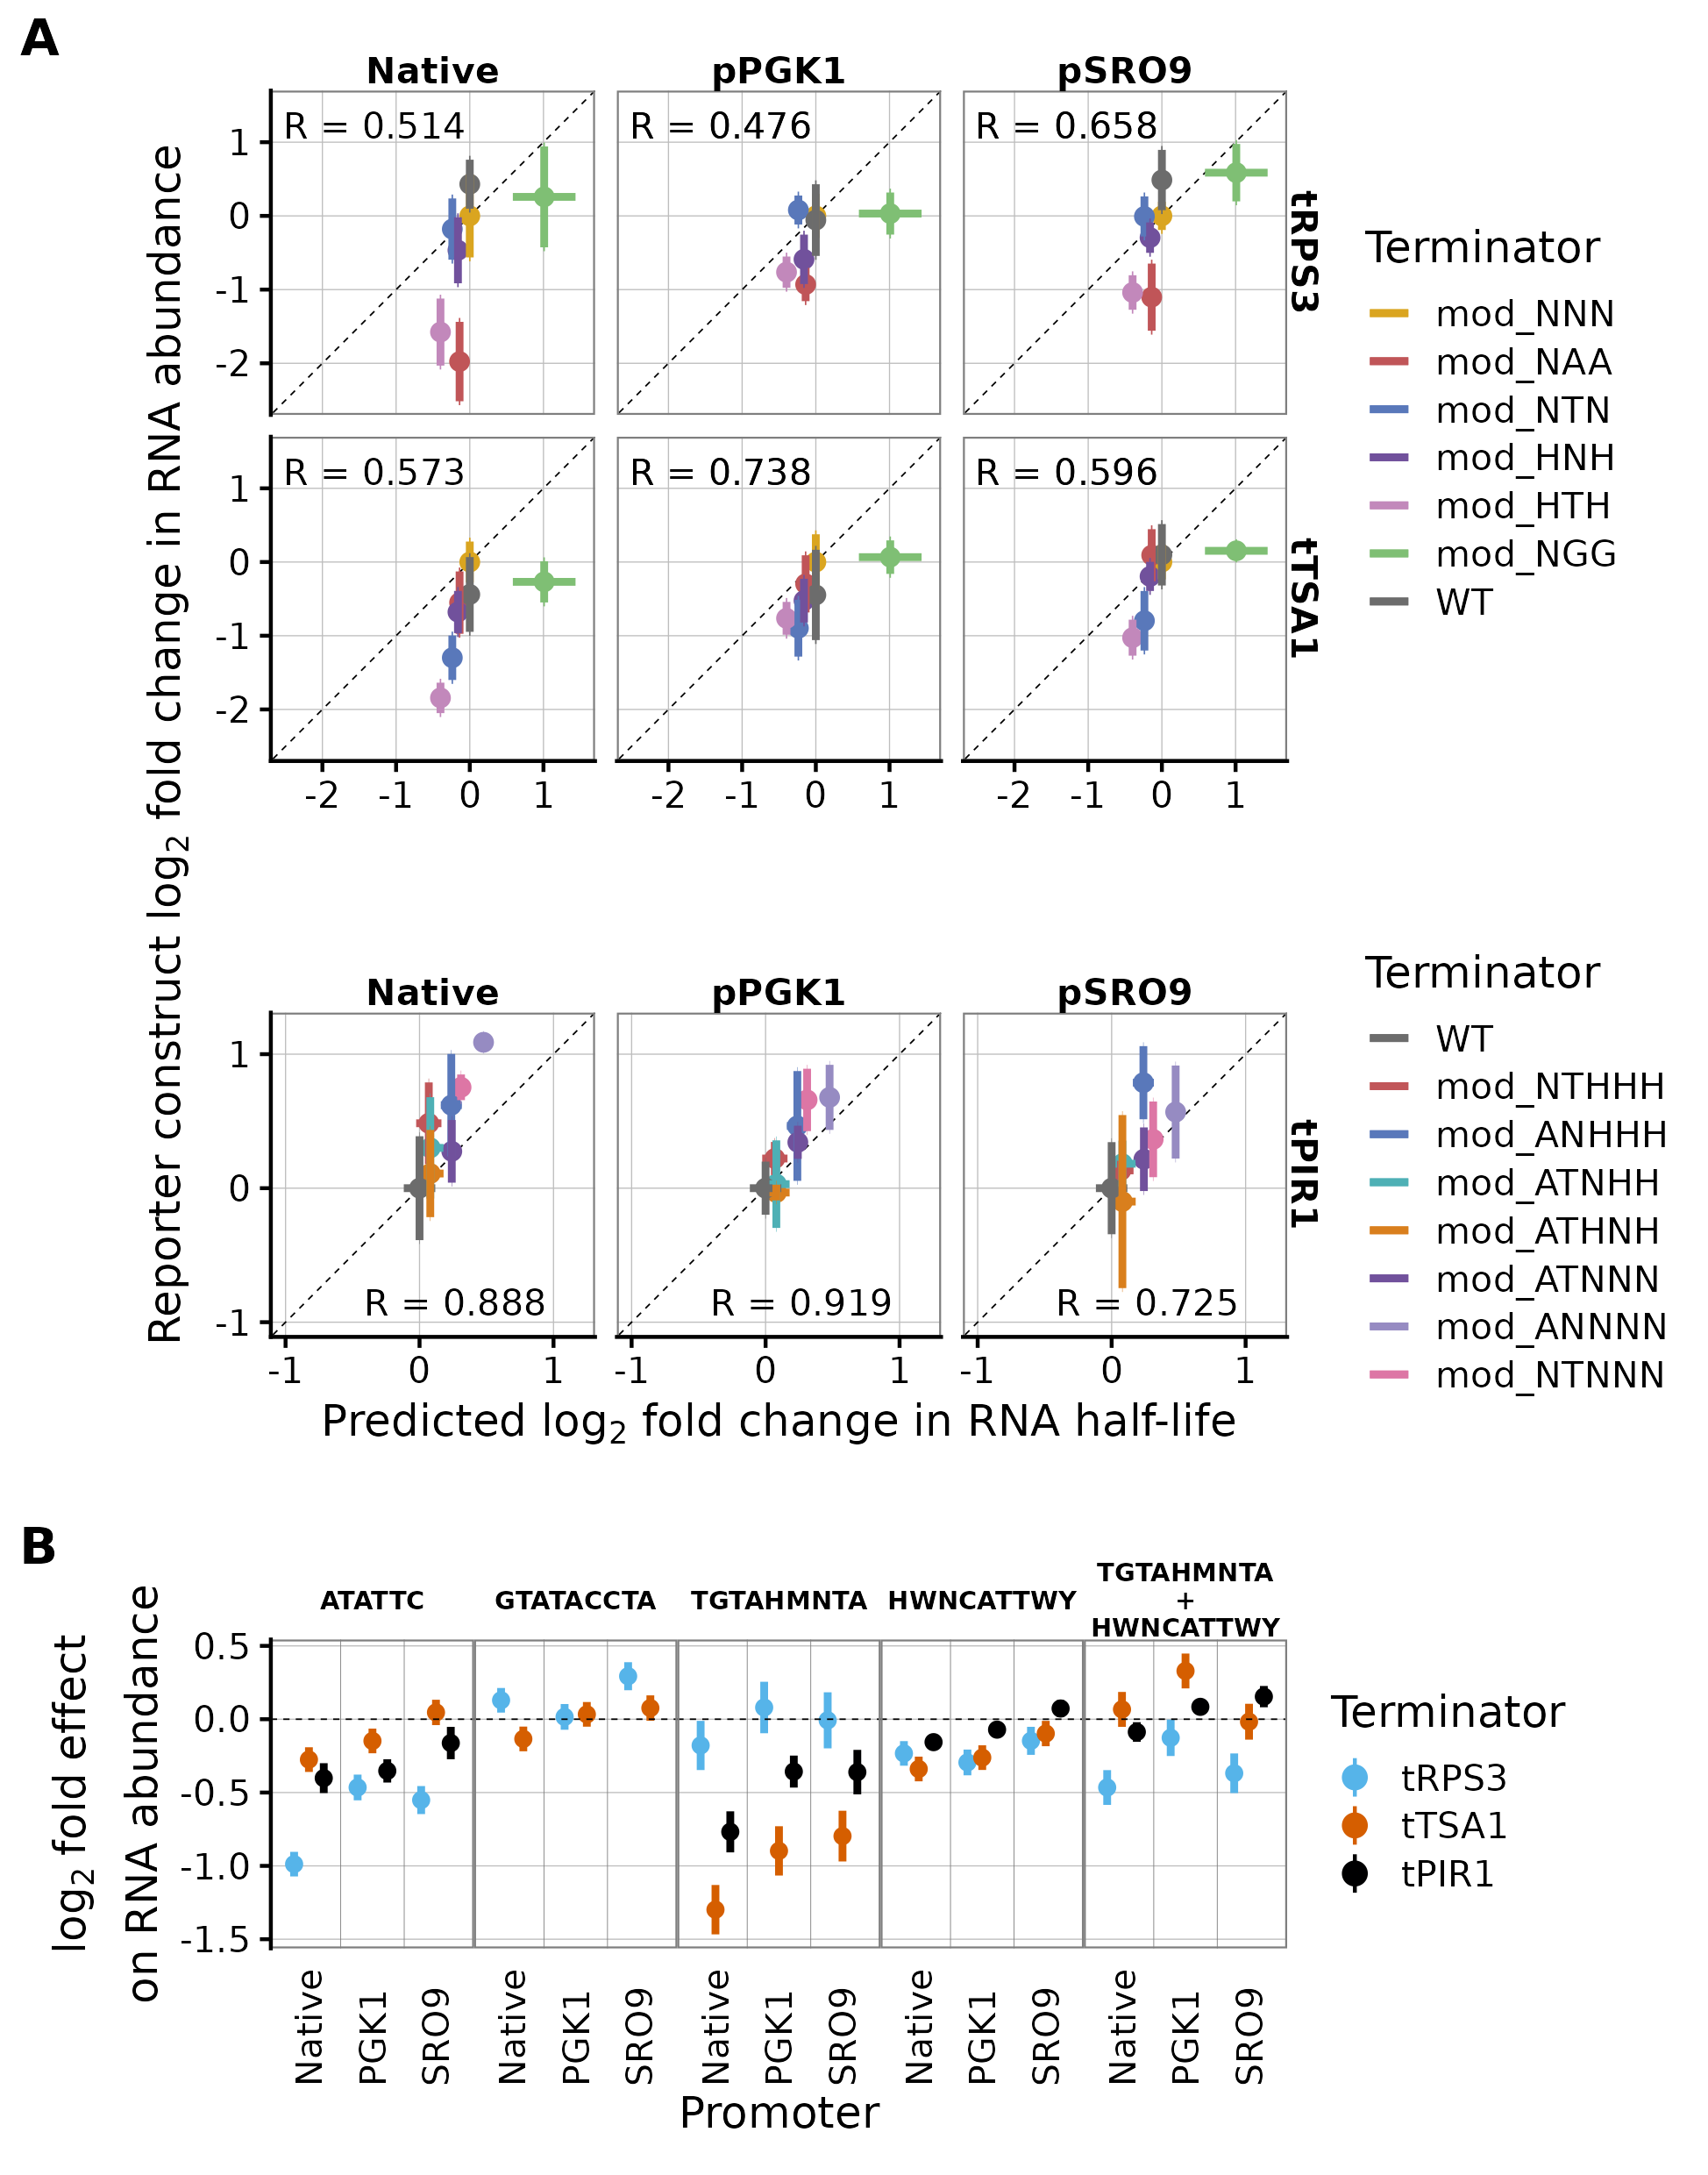
\includegraphics[width=0.85\linewidth]{qPCR_model_coef_and_pred_vs_exp_abund} 

}

\caption[Promoter and terminator context alter the regulatory effect of motifs.]{\textbf{Promoter and terminator context alter the regulatory effect of motifs.} (\textbf{A}) Predicted change in transcript abundance inferred from transcriptome-wide motif contributions to half-life, compared to RT-qPCR measurements of reporter transcript abundance. The y-axis shows statistical summaries (mean and standard error) of 6 replicates for data shown in figures 4 and 5. The fold change is relative to the mod\_NNN construct in each promoter-terminator pairing for the tRPS3 and tTSA1 sets, and relative to the WT constructs for tPIR1 sets. Native promoter panels show the promoter paired with the terminator from the same set, e.g. pRPS3 with tRPS3. (\textbf{B}) Motif contributions to fold changes in mRNA abundance for reporter constructs with different promoter and terminator contexts. This is calculated by a linear model with a coefficient for the effect of each motif in each set, applied to $\Delta Cq$ against 3 reference genes. The last column shows the interaction term between TGTAHMNTA and HWNCATTWY.}\label{fig:hlife-predict-vs-abundance-and-motif-context-dependence}
\end{figure}

\subsection{Inserting motifs into terminators shifts poly(A) site usage downstream}

We next mapped poly(A) site usage in a subset of reporter constructs, for 2 reasons.
First, changes in poly(A) site usage might mean that motifs placed in our reporters were unintentionally absent from the mature mRNA.
Second, we wanted to know if motif effects on mRNA abundance might be due to changes in the poly(A) site usage.
We chose three constructs with large effect sizes in the qPCR results: mod\_NAA, mod\_HTH and mod\_NTN, together with WT and mod\_NNN controls, within three promoter-terminator contexts: pRPS3-tRPS3, pPGK1-tRPS3 and pTSA1-tTSA1.
For these constructs we performed paired-ends sequencing of 3' mRNA-Seq libraries following QuantSeq protocol (\parencite{Moll2014} and see methods).
Read 1 allows precise inference of poly(A) site position while read 2 generally overlaps the CDS and allows distinguishing terminators in native loci from reporter constructs.
We mapped the reads to genome sequences extended by the relevant reporter plasmid sequence.

We detected 1000s of reads on each reporter construct, which is enough to quantify expression confidently as well as to assign poly(A) sites.
We checked that counts of all other RNAs are highly correlated between samples, giving us confidence that changes in construct detection are meaningful (Supplementary Figure \ref{fig:rnaseq-QC-correlation}).
Transcript abundance, relative to mod\_NNN, for most constructs correlates strongly with qPCR results (Figure \ref{fig:quantseq-polyA-site-usage}A).
However, some constructs were detected as more abundant by RNA-seq for reasons that are unclear.

We display the poly(A) sites as the cumulative fraction of poly(A)-site reads mapped at each location downstream of construct stop codons, out of all reads mapped to the terminator (Figure \ref{fig:quantseq-polyA-site-usage}B).
We confirmed that in other genes the poly(A) site locations were highly reproducible across samples, giving us confidence that changes in reporter poly(A) sites are meaningful (Supplementary Figure \ref{fig:rnaseq-QC-QuantSeq-and-5PSeq-genomic-polyA}).
Poly(A) sites are in the same relative positions in native loci and the constructs with wild-type terminator (Supplementary Figure \ref{fig:rnaseq-QC-genomic-vs-plasmid-polyA}).
Then, we compared 3'end positions of reads between modified and wild-type reporter constructs to determine the poly(A) site usage.
In both wild-type and mod\_NNN tTSA1 constructs, the relative usage of major poly(A) sites does not significantly change (Site 1 p-value = 0.068 and Site 2 p-value = 1).
Surprisingly, tRPS3 mod\_NNN constructs appear to be using a novel upstream poly(A) site, that appears in about \(50%
\) percent of reads and is located upstream of the 3rd motif insertion site (Site 1 p-value = 0.016; Figure \ref{fig:quantseq-polyA-site-usage}B).

Next, we compared changes in poly(A) site usage between constructs with different inserted motifs.
We highlight the 2 major poly(A) sites for the tRPS3 constructs and 2 for the tTSA1 constructs (black vertical lines on the mod\_NNN constructs in Figure \ref{fig:quantseq-polyA-site-usage}B) and track the cumulative fraction of reads upstream of each major site.
However, for tRPS3 constructs there is a distinct shift to downstream poly(A) sites in constructs with verified, rather than random, motifs inserted.
There are also smaller differences in poly(A) site usage between constructs with different motifs (Supplementary Figure \ref{fig:quantseq-polyA-site-usage}C, Supplementary Table \ref{tab:polya-usage-effect-table}).

\begin{figure}[p]

{\centering 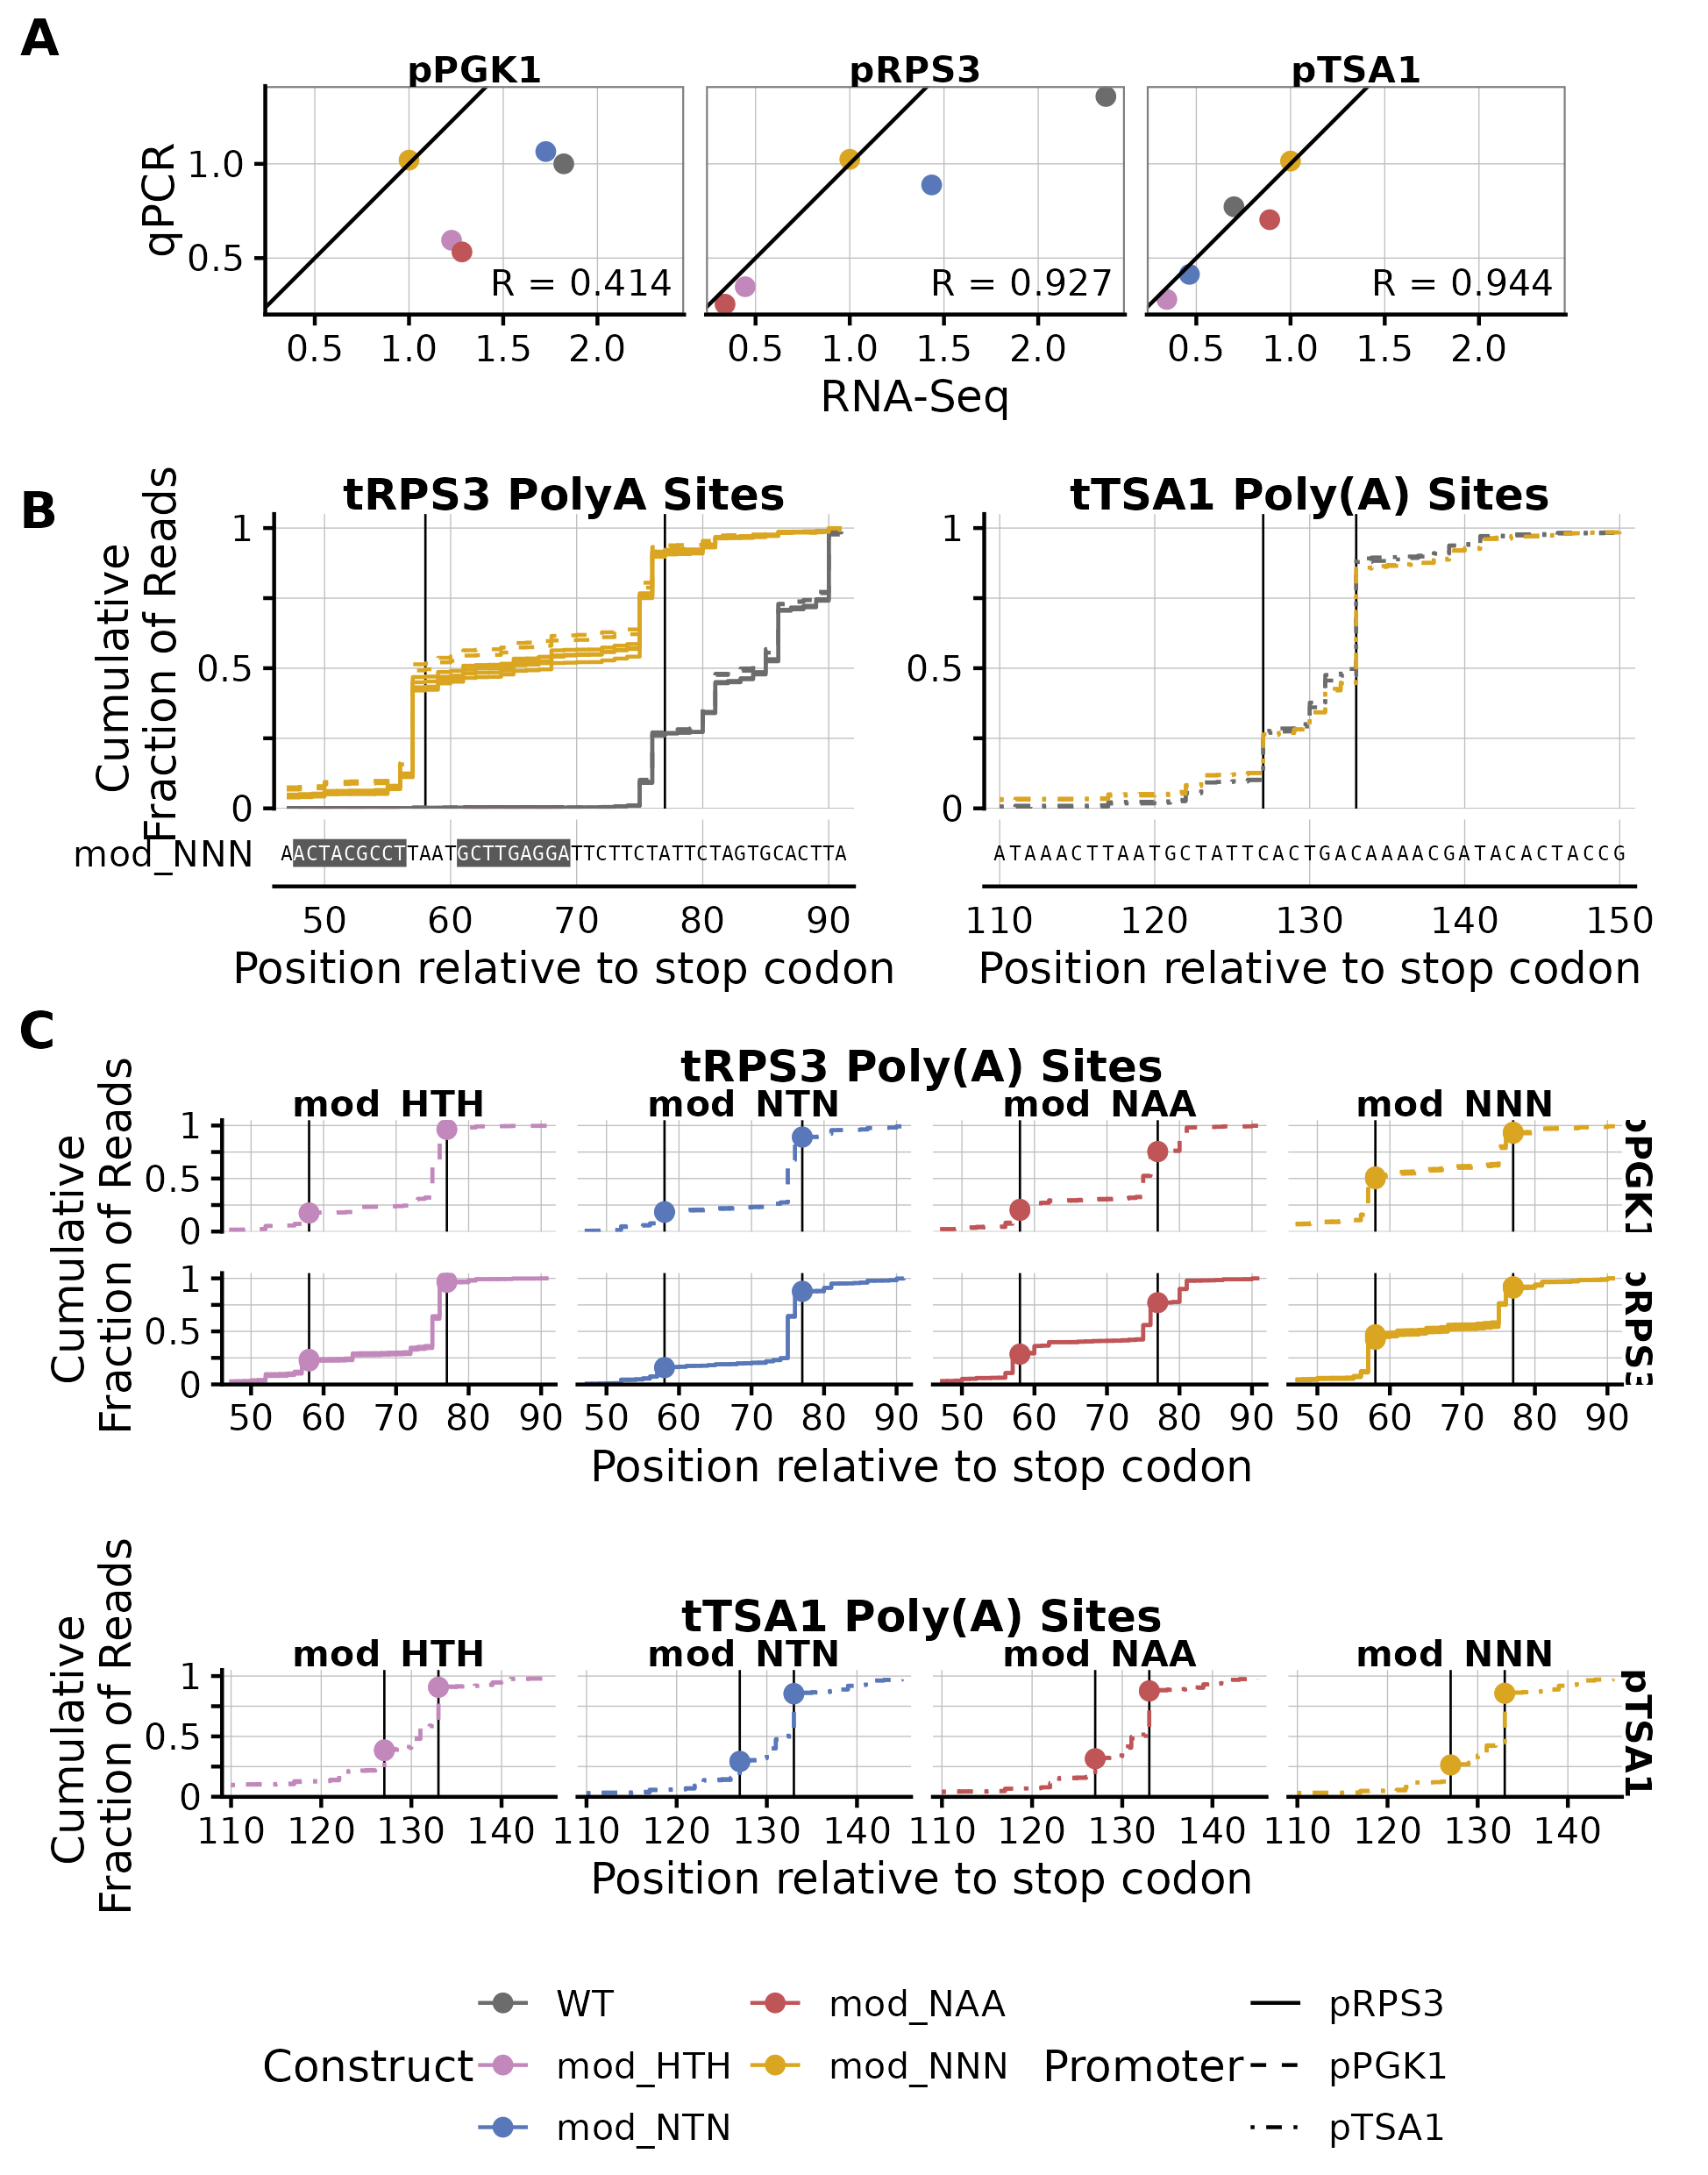
\includegraphics[width=0.85\linewidth]{polya_usage_plot_QuantSeq.png} 

}

\caption[Inserting motifs into RPS3 and TSA3 terminators changes 3'UTR length.]{\textbf{Inserting motifs into RPS3 and TSA3 terminators changes 3'UTR length.} A subset of constructs were chosen to investigate changes in poly(A) site usage: WT, mod\_NNN, mod\_NTN, mod\_NAA, and mod\_HTH; within three promoter-terminator contexts: pRPS3-tRPS3, pPGK1-tRPS3, and pTSA1-tTSA1. (\textbf{A}) Comparison of construct transcript abundance as independently measured by qPCR and RNA-Seq assays. Transcript abundance was normalised to the median abundance of  plasmid URA3, genomic PGK1, and RPS3 or TSA1 transcripts for each construct. Fold change is relative to the mod\_NNN construct in each promoter-terminator context. The black diagonal line represents the expected values if RNAseq and qPCR results correlated perfectly. (\textbf{B}) Cumulative count of reads mapped downstream of WT (grey) and mod\_NNN (golden) construct stop codons as fraction of total reads mapped to the constructs terminator. The x-axis shows the terminator sequence of the mod\_NNN construct with inserted random motifs highlighted with a black background. WT reads have been shifted downstream to align with the mod\_NNN sequence by accounting for motif insertion sites. Major poly(A) sites have been highlighted by a black vertical line. (\textbf{Left}) shows the poly(A) sites for the pRPS3-tRPS3 and pPGK1-tRPS3 promoter-terminator constructs. (\textbf{Right}) shows the same for the pTSA1-tTSA1 constructs. (\textbf{C}) Similar to Figure \textbf{B} but with each motif insertion construct plotted separately. Columns designate cumulative plots from different terminator constructs and rows designate cumulative plots from different promoter contexts.}\label{fig:quantseq-polyA-site-usage}
\end{figure}

We then asked whether modifications in the 3'-UTR region impact 5'-3' degradation following mRNA decapping, using the 5PSeq method targeted to the 3'-end regions of mRNA \parencite{Pelechano2016}.
5PSeq can detect changing ribosome dynamics through 5'-3' co-translational degradation, however, the novel modification to 5Pseq here uses an anchored oligo(dT) reverse primer so detects only the poly(A)-site proximal region of the mRNA instead of the entire coding sequence.
The 5Pseq counts per gene are highly reproducible between samples (Supplementary Figure \ref{fig:rnaseq-QC-correlation}B), and the abundances of reporter mRNAs from different constructs correlate well between 5PSeq and QuantSeq data (Supplementary Figure \ref{fig:rnaseq-QC-correlation}C).
Our 5PSeq data finds no detectable changes in 5'-phosphorylated intermediates between wild-type and modified reporter constructs, and thus does not indicate detectable changes in ribosome dynamics near the 3' end of transcripts (Supplementary Figure \ref{fig:rnaseq-QC-genomic-vs-plasmid-polyA}, \ref{fig:combined-5p-end-read-plot}).
It does confirm the behaviour of the inserted motifs correlates with qPCR results and that an upstream alternative polyadenylation site is introduced in the tRPS3 constructs (Supplementary Figure \ref{fig:polyA-site-usage-5Pseq}).
Moreover, the poly(A) site distribution for each construct matches that obtained from QuantSeq data, suggesting that 3'-UTR isoforms are not differentially degraded using this pathway regardless of the motifs inserted (Supplementary Figure \ref{fig:relative-polya-counts}, Supplementary Table \ref{tab:polya-usage-effect-5PSeq-table}).
Finally, the abundances of different reporter mRNAs from different constructs correlate well between
5PSeq and QuantSeq data (Supplementary Figure \ref{fig:rnaseq-QC-correlation}C).

Overall, poly(A) site mapping showed that most reporter mRNAs retained the expected poly(A) site and motifs, except for a new alternative poly(A) site in tRPS3 mod\_NNN constructs.
This highlights the potential for unexpected consequences from composing cis-regulatory elements, even when introducing ``random'' insertions of no known function.


\section{Chapter 4 Conclusions}

This work explores the limitations of composability in cis-regulatory elements. 
The effects of interacting promoter and terminator regions have been well documented in the synthetic biology literature \parencite{Ito2013, Dhillon2020}. 
However, the narrative describes this degree of unpredictably as a nuisance obstructing the creation of reliable genetic circuits and high value products \parencite{Kittleson2012}. 
The focus on creating reliable components with predictable contributions overlooks the evidence for a far more complex picture of regulatory mechanisms that is biologically interesting in itself. 

We first build on current literature to show the variability in contribution to gene expression from terminators from known regulatory genes in response to differing coding regions and promoters. 
As expected, our protein fluorescence results show up to 100 fold changes by promoter choice alone and then up to 5 fold by terminator choice.
Then, we highlight significant changes in several terminator contributions to gene expression. 
We highlight the quantitative limitations of the assumption of composability with 1.5 fold change in the relative effect of terminators depending on coding sequence and promoter choice.


We extend our understanding of this unexplained behaviour by testing the regulatory behaviour of cis-regulatory elements within the terminator, namely short sequence motifs within the 3'UTR.
We show that the analysis of published data sets can enhance experimental design by building on previous work by \cite{Cheng2017} and shortlisting several prospective 3'UTR motifs using a linear model predicting half life.
Inserting or removing these motifs from three native host terminators, we showed that three of the four motifs performed as expected on their affect on transcript levels as measure by qPCR.
Furthermore, the magnitude of their contributions changed for all motifs across promoter and host terminator. 
TGTAHMNTA has no measurable effect when inserted into tRPS3 but has the expected effect in tTSA1, ATATTC has the expected effect in tRPS3 but little effect in tTSA1, and HWNCATTWY can either decrease or increase mRNA levels when removed from tPIR1, depending on the promoter.
Also, the two tPIR1 constructs with different mutated HWNCATTWY motifs had different expression levels suggesting HWNCATTWY has a position-dependent effect. 
However, the exact sequences of the two HWNCATTWY motif instances did also differ by 4 nucleotides.
Interestingly, when two motifs were inserted/removed together their combined contribution also changed across contexts.

RNA-Seq results confirmed our conclusions on the effect of motif insertions on gene expression. pRPS3-tRPS3 and pTSA1-tTSA1 constructs show similar relative abundances in the qPCR results as the RNA-Seq results. 
However, pPGK1-tRPS3 results are skewed due to the unexpected low abundance of mod NNN constructs in the RNA-Seq results, which all other constructs are normalised to.
We investigated if positional effects could be contributing to the differing behaviour. 
In TSA1 the poly(A) site usage was unchanged between WT and the insertion constructs. 
However, in RPS3 a new alternative poly(A) site had been unintentionally introduced in between insertion sites 2 and 3 for all constructs. 
Although we tried to avoid altering elements affect poly(A) sites in native terminators, the creation of novel poly(A) site is likely due to the inserted motifs extending the distance between the efficiency elements and the native poly(A) sites.
Another possible explanation for the novel poly(A) site is that motifs 2 and 3 were inserted into a conserved element of tRPS3, as detected by pHastCons \parencite{Siepel2005}.
As TGTAHMNTA and ATATTC are both inserted in site 2 (and ATATTC is also inserted into site 3) there is a chance that their behaviour is affected in RPS3.
Interestingly, despite all tTSA1 constructs having 2 ATATTC motifs they have less effect on transcript level than in tRPS3, which has just one copy in nearly 50\% of transcripts.
ATATTC could need to be close to Poly(A) site, so the novel poly(A) site in tRPS3 is actually beneficial, but ATATTC is not near poly(A) site in tPIR1 and still has greater effect than in tTSA1.
Meanwhile TGTAHMNTA could be nullified by the proximity to the novel poly(A) site.
Although, it is interesting that only in tRPS3 is the combined effect of HWNCATTWY and TGTAHMNTA synergistic.
Further constructs with insertion sites across the terminators are required to confirm the positional effects.

We believe that the study of interactions between cis-regulatory elements is an understudied research area. 
It promises to improve the predictability of contributions to gene expression required to enhance the design of synthetic pathways and is also a fruitful region for discovering novel mechanisms through which cell regulate their expression. 
We have shown that changes in contributions according to context can affect cis-regulatory elements such as motifs as well as regions like terminators. 
We have also shown that changes in contributions due to co-occuring motifs can be measured using linear interaction terms trained on qPCR data. 
Our work designing suitable insertion sites into host terminators to detect these changes also offers a framework to inspect context effects on cis-regulatory elements at scale. 
Finally, this work also showcases the usefulness of our R package tidyqpcr as our analysis of complex, multi-experimental qPCR data is entirely open, reproducible and quality controlled.

\end{document}